\clearpage %&latex
\documentclass[a4paper]{article}

\frenchspacing

\usepackage[cp1250]{inputenc}
\usepackage[czech]{babel}

\usepackage{a4wide}
\usepackage{amsmath, amsthm, amssymb, amsfonts}
\usepackage[mathcal]{eucal}
\usepackage{graphicx}
\usepackage{url}
\usepackage{color}
\usepackage{wrapfig}
\usepackage{capt-of}
\usepackage{float}



% sirka a vyska textu nastavena jako papir, vsechny okraje vynulovany a pridano 20pt na kazdou stranu
% horizontalni rozmery
\setlength{\textwidth}{\paperwidth}
\addtolength{\textwidth}{-40pt}
\addtolength{\hoffset}{-1in}
\addtolength{\hoffset}{20pt}
\setlength{\oddsidemargin}{0in}
\setlength{\marginparsep}{0in}
% vertikalni rozmery
\setlength{\textheight}{\paperheight}
\addtolength{\textheight}{-60pt}
\addtolength{\voffset}{-1in}
\addtolength{\voffset}{20pt}
\setlength{\topmargin}{0in}
\setlength{\headheight}{0in}
\setlength{\headsep}{0in}


%Obrazek na miste
%pouziti
%%\obrazeknahore{adresa}{popisek}{label}
\long\def\obrazeknahore#1#2#3 {

\begin{figure}[t]
    \centering
    \includegraphics[width=0.8\textwidth]{#1}
    
    \caption{#2}
    \label{#3}
    
\end{figure}

}


%==========================================
%PEKELNA MAKRA NA ZAROVNANI OBRAZKU DOPRAVA

\makeatletter


%tohle je makro, ktere mi dovoluje obtekani i u kratkych environmentu
%ABSOLUTNE nechapu, jak to funguje, ale funguje to
%viz http://tex.stackexchange.com/questions/26078/ 
\def\odrovnej{\@@par
\ifnum\@@parshape=\z@ \let\WF@pspars\@empty \fi % reset `parshape'
\global\advance\c@WF@wrappedlines-\prevgraf \prevgraf\z@
\ifnum\c@WF@wrappedlines<\tw@ \WF@finale \fi}

\makeatother



%---
%makro, co da obrazek doprava a ostatni text ho obteka
%(bez toho predchazejiciho makra to ale poradne nebeha)
%pouziti:
%\obrazekvpravo{adresa}{popisek}{label}{procento sirky}
\long\def\obrazekvpravo#1#2#3#4{

\setlength\intextsep{-20pt}

    \begin{wrapfigure}{r}{#4\textwidth}
      \begin{center}
          \vspace{-10pt}
          
        \includegraphics[width=#4\textwidth]{#1}
        \vspace{-10pt}
        
      \end{center}
      
      \caption{#2}
      \label{#3}
      
      
    \end{wrapfigure}

\setlength\intextsep{0pt}

    
}




%---
%makro pro pripady, kdy wrapfigure neco mrsi
%je to docela pekelne
%je nutne mu dat jak text vpravo, tak text vlevo
%a nevim, jestli bude 100% fungovat, ale doufam, ze jo

%pouziti:
%\obrazekvpravominipage{adresa}{popisek}{label}{procento sirky}{1 - procento sirky}{text vlevo}
\long\def\obrazekvpravominipage#1#2#3#4#5#6{

\noindent\begin{minipage}{#5\linewidth}
\vspace{0pt}
#6
\end{minipage}
\hspace{0.5cm}
\noindent\begin{minipage}{#4\linewidth}
\vspace{0pt}
\centering
\includegraphics[width=0.9\textwidth]{#1}
\captionof{figure}{#2}
\label{#3}
\end{minipage}

}

%KONEC PEKELNYCH MAKER
%=====================

% makra pro poznamku u vyrokove a predikatove logiky
\def\vl{ -- ve v�rokov� logice}
\def\pl{ -- v predik�tov� logice}


%Vacsina prostredi je dvojjazicne. V pripade, ze znenie napr pozorovania je pisane po slovensky, malo by byt po slovensky aj oznacenie.

\newenvironment{pozadavky}{\pagebreak[2]\noindent\textbf{Po�adavky}\par\noindent\leftskip 10pt}{\odrovnej\par\bigskip}
\newenvironment{poziadavky}{\pagebreak[2]\noindent\textbf{Po�iadavky}\par\noindent\leftskip 10pt}{\odrovnej\par\bigskip}


\newenvironment{definiceSkull}{\pagebreak[2]\noindent\textbf{$\bigstar$ Definice}\par\noindent\leftskip 10pt}{\odrovnej\par\bigskip}
\newenvironment{definiceNSkull}[1]{\pagebreak[2]\noindent\textbf{$\bigstar$ Definice~}\emph{(#1)}\par\noindent\leftskip 10pt}{\odrovnej\par\bigskip}

\newenvironment{definice}{\pagebreak[2]\noindent\textbf{Definice}\par\noindent\leftskip 10pt}{\odrovnej\par\bigskip}
\newenvironment{definiceN}[1]{\pagebreak[2]\noindent\textbf{Definice~}\emph{(#1)}\par\noindent\leftskip 10pt}{\odrovnej\par\bigskip}
\newenvironment{definicia}{\pagebreak[2]\noindent\textbf{Defin�cia}\par \noindent\leftskip 10pt}{\odrovnej\par\bigskip}
\newenvironment{definiciaN}[1]{\pagebreak[2]\noindent\textbf{Defin�cia~}\emph{(#1)}\par\noindent\leftskip 10pt}{\odrovnej\par\bigskip}

\newenvironment{vetaSkull}{\pagebreak[2]\noindent\textbf{$\bigstar$ V�ta}\par\noindent\leftskip 10pt}{\odrovnej\par\bigskip}
\newenvironment{vetaNSkull}[1]{\pagebreak[2]\noindent\textbf{$\bigstar$ V�ta~}\emph{(#1)}\par\noindent\leftskip 10pt}{\odrovnej\par\bigskip}

\newenvironment{pozorovani}{\pagebreak[2]\noindent\textbf{Pozorov�n�}\par\noindent\leftskip 10pt}{\odrovnej\par\bigskip}
\newenvironment{pozorovanie}{\pagebreak[2]\noindent\textbf{Pozorovanie}\par\noindent\leftskip 10pt}{\odrovnej\par\bigskip}
\newenvironment{poznamka}{\pagebreak[2]\noindent\textbf{Pozn�mka}\par\noindent\leftskip 10pt}{\odrovnej\par\bigskip}
\newenvironment{poznamkaN}[1]{\pagebreak[2]\noindent\textbf{Pozn�mka~}\emph{(#1)}\par\noindent\leftskip 10pt}{\odrovnej\par\bigskip}
\newenvironment{lemma}{\pagebreak[2]\noindent\textbf{Lemma}\par\noindent\leftskip 10pt}{\odrovnej\par\bigskip}
\newenvironment{lemmaN}[1]{\pagebreak[2]\noindent\textbf{Lemma~}\emph{(#1)}\par\noindent\leftskip 10pt}{\odrovnej\par\bigskip}
\newenvironment{veta}{\pagebreak[2]\noindent\textbf{V�ta}\par\noindent\leftskip 10pt}{\odrovnej\par\bigskip}
\newenvironment{vetaN}[1]{\pagebreak[2]\noindent\textbf{V�ta~}\emph{(#1)}\par\noindent\leftskip 10pt}{\odrovnej\par\bigskip}
\newenvironment{vetaSK}{\pagebreak[2]\noindent\textbf{Veta}\par\noindent\leftskip 10pt}{\odrovnej\par\bigskip}
\newenvironment{vetaSKN}[1]{\pagebreak[2]\noindent\textbf{Veta~}\emph{(#1)}\par\noindent\leftskip 10pt}{\odrovnej\par\bigskip}

\newenvironment{dusledek}{\pagebreak[2]\noindent\textbf{D�sledek}\par\noindent\leftskip 10pt}{\odrovnej\par\bigskip}
\newenvironment{dosledok}{\pagebreak[2]\noindent\textbf{D�sledok}\par\noindent\leftskip 10pt}{\odrovnej\par\bigskip}

\newenvironment{dokaz}{\pagebreak[2]\noindent\leftskip 10pt\textbf{D�kaz}\par\noindent\leftskip 10pt}{\odrovnej\par\bigskip}
\newenvironment{dukaz}{\pagebreak[2]\noindent\leftskip 10pt\textbf{D�kaz}\par\noindent\leftskip 10pt}{\odrovnej\par\bigskip}

\newenvironment{ideadukazu}{\pagebreak[2]\noindent\leftskip 10pt\textbf{Idea d�kazu}\par\noindent\leftskip 10pt}{\odrovnej\par\bigskip}


\newenvironment{priklad}{\pagebreak[2]\noindent\textbf{P��klad}\par\noindent\leftskip 10pt}{\odrovnej\par\bigskip}
\newenvironment{prikladN}[1]{\pagebreak[2]\noindent\textbf{P��klad~}\emph{(#1)}\par\noindent\leftskip 10pt}{\odrovnej\par\bigskip}

\newenvironment{prikladSK}{\pagebreak[2]\noindent\textbf{Pr�klad}\par\noindent\leftskip 10pt}{\odrovnej\par\bigskip}
\newenvironment{priklady}{\pagebreak[2]\noindent\textbf{P��klady}\par\noindent\leftskip 10pt}{\odrovnej\par\bigskip}
\newenvironment{prikladySK}{\pagebreak[2]\noindent\textbf{Pr�klady}\par\noindent\leftskip 10pt}{\odrovnej\par\bigskip}

\newenvironment{algoritmusN}[1]{\pagebreak[2]\noindent\textbf{Algoritmus~}\emph{(#1)}\par\noindent\leftskip 10pt}{\odrovnej\par\bigskip}
%obecne prostredie, ktore ma vyuzitie pri specialnych odstavcoch ako (uloha, algoritmus...) aby nevzniklo dalsich x prostredi
\newenvironment{obecne}[1]{\pagebreak[2]\noindent\textbf{#1}\par\noindent\leftskip 10pt}{\odrovnej\par\bigskip}

\newenvironment{report}{\pagebreak[2]\noindent\textbf{Report}\em\par\noindent\leftskip 10pt}{\par\bigskip}

%\newenvironment{reportN}[1]{\pagebreak[2]\noindent\textbf{Report~}\emph{(#1)}\emph\par\noindent\leftskip 10pt}{\odrovnej\par\bigskip}
\newenvironment{reportN}[1]{\pagebreak[2]\noindent\textbf{Report~}\emph{(#1)}\em\par\noindent\leftskip 10pt}{\odrovnej\par\bigskip}

\newenvironment{penumerate}{
\begin{enumerate}
  \setlength{\itemsep}{1pt}
  \setlength{\parskip}{0pt}
  \setlength{\parsep}{0pt}
  %\setlength{\topsep}{200pt}
  \setlength{\partopsep}{200pt}
}{\end{enumerate}}

\def\pismenka{\numberedlistdepth=2} %pouzit, ked clovek chce opismenkovany zoznam...

\newenvironment{pitemize}{
\begin{itemize}
  \setlength{\itemsep}{1pt}
  \setlength{\parskip}{0pt}
  \setlength{\parsep}{0pt}
}{\end{itemize}}

%\definecolor{gris}{gray}{0.95}
\newcommand{\ramcek}[2]{\begin{center}\fcolorbox{white}{gris}{\parbox{#1}{#2}}\end{center}\par}
 \clearpage
\title{\LARGE Učební texty k státní bakalářské zkoušce \\ Obecná informatika \\ Algoritmy a datové struktury}
\begin{document}
\maketitle
\newpage
\setcounter{section}{2}
\section{Algoritmy a datové struktury}
\begin{pozadavky}
\begin{pitemize}
\item Časová složitost algoritmů, složitost v nejhorším a průměrném případě.
\item Třídy složitosti P a NP, převoditelnost, NP-úplnost.
\item Metoda ,,rozděl a panuj'' - aplikace a analýza složitosti.
\item Binární vyhledávací stromy, vyvažování, haldy.
\item Hašování.
\item Sekvenční třídění, porovnávací algoritmy, přihrádkové třídění, třídící sítě.
\item Grafové algoritmy - prohledávání do hloubky a do šířky, souvislost, topologické třídění, nejkratší cesta, kostra grafu, toky v sítích.
\item Tranzitivní uzávěr.
\item Algoritmy vyhledávání v textu.
\item Algebraické algoritmy - DFT, Euklidův algoritmus.
\item Základy kryptografie, RSA, DES.
\item Pravděpodobnostní algoritmy - testování prvočíselnosti.
\item Aproximační algoritmy.
\end{pitemize}
\end{pozadavky}
\subsection{�asov� slo�itost algoritm�, slo�itost v nejhor��m a pr�m�rn�m p��pad�}


\begin{e}{Definice}{0}{�asov� slo�itost}
  \textbf{�asovou slo�itost�} algoritmu rozum�me z�vislost jeho �asov�ch n�rok� na
  velikosti konkr�tn�ch vstupn�ch dat. Analogicky se definuje i \textbf{pam�ov�
  slo�itost}. Dobu zpracov�n� �lohy o velikosti $n$ zna��me $T(n)$\\
  �asovou slo�itost �asto zkoum�me z n�kolik hledisek:
  \begin{pitemize}
    \item \textbf{v nejhor��m p��pad�}~-- maxim�ln� po�et operac� pro n�jak� data, 
    \item \textbf{v nejlep��m p��pad�}~-- minim�ln� po�et operac� pro n�jak� data,
    \item \textbf{v pr�m�rn�m (o�ek�van�m) p��pad�}~-- pr�m�r pro v�echna mo�n�
  vstupn� data (n�kdy t� st�edn� hodnota n�hodn� veli�iny $T(n)$).
  \end{pitemize}

  \begin{e}{Pozn�mka}{0}{0}
  Jako jednu \uv{operaci}, nebo-li \emph{krok algoritmu} rozum�me jednu element�rn� 
  operaci n�jak�ho abstraktn�ho stroje (nap�. Turingova stroje), proveditelnou v 
  konstantn�m �ase. Intuitivn�
  je mo�n� ch�pat to jako n�kolik operac� po��ta�e, kter� dohromady netrvaj� v�ce,
  ne� n�jakou pevn� danou dobu.
  \end{e}
\end{e}

\begin{e}{Pozn�mka}{0}{0}
  �asov� slo�itost probl�mu je rovna slo�itosti nejlep��ho algoritmu �e��c�ho
  dan� probl�m.
\end{e}


\subsubsection*{Asymptotick� slo�itost}

\begin{e}{Definice}{0}{0}
  �ekneme, �e funkce $f(n)$ je \textbf{asymptoticky men�� nebo rovna} ne� $g(n)$,
  zna��me $f(n)$ je $O(g(n))$, pr�v� tehdy, kdy�
  $$ \exists c>0\ \exists n_0\ \forall n>n_0: 0 \leq f(n) \leq c \cdot g(n)$$
  Funkce $f(n)$ je \textbf{asymptoticky v�t�� nebo rovna} ne� $g(n)$, zna��me
  $f(n)$ je $\Omega(g(n))$, pr�v� tehdy, kdy�
  $$ \exists c>0\ \exists n_0\ \forall n>n_0: 0 \leq c \cdot g(n) \leq f(n)$$
  Funkce $f(n)$ je \textbf{asymptoticky stejn�} jako $g(n)$, zna��me $f(n)$ je
  $\Theta(g(n))$, pr�v� tehdy, kdy�
  $$ \exists c_1,c_2>0\ \exists n_0\ \forall n>n_0: 0 \leq c_1 \cdot g(n) \leq
  f(n) \leq c_2 \cdot g(n)$$
\end{e}

\begin{e} {Pozn�mka}{0}{0}
  Asymptotick� slo�itost zkoum� chov�n� algoritm� na \uv{velk�ch} datech a dle
  jejich slo�itosti je za�azuje do skupin (polynomi�ln�, exponenci�ln�\dots).
  P�i zkoum�n� se zanedb�vaj� aditivn� a multiplikativn� konstanty. 
\end{e}

\subsubsection*{Amortizovan� slo�itost}

\begin{e}{Definice}{0}{Amortizovan� slo�itost}
  \emph{Amortizovan� �asov� slo�itost} po��t� pr�m�rn� �as na jednu operaci p�i proveden�
  posloupnosti operac�. Pou��v� se typicky pro po��t�n� �asov� slo�itosti operac�
  nad datov�mi strukturami. D�v� realisti�t�j�� horn� odhad slo�itosti
  posloupnosti operac�, ne� po��t�n� s nejhor��m p��padem u ka�d� operace.
\end{e}

\begin{obecne}{Agrega�n� metoda}
  Spo��t�me (nejhor�� mo�n�) �as $T(n)$ pro posloupnost operac�. Amortizovan� cena
  jedn� operace je potom $\frac{T(n)}{n}$.
\end{obecne}

\begin{obecne}{��etn� metoda}
  Od ka�d� operace \uv{vybereme} ur�it� \uv{obnos}, ze kter�ho \uv{zaplat�me} za
  danou operaci a pokud n�co zbude, d�me to na ��et. Pokud je operace dra��� ne�
  kolik je jej� obnos, tak pot�ebn� rozd�l vybereme z ��tu. Z�statek na ��tu
  mus� b�t st�le nez�porn�. Pokud usp�jeme, tak \uv{obnos} = amortizovan� cena
  jedn� operace.
\end{obecne}

\begin{e}{Pozn�mka}{0}{0}
  Jde o to, �e n�kter� operace m��e trvat kr�tce, ale \uv{rozh�e} datovou
  strukturu, tak�e n�sleduj�c� operace pot�ebuj� v�c �asu. Nebo naopak trv�
  dlouho a datovou strukturu \uv{uspo��d�}, tak�e ostatn� operace jsou krat��.
\end{e}

\subsection{T��dy slo�itosti P a NP, p�evoditelnost, NP-�plnost}

TODO: doplnit, tohle asi nestaci na pohodovou zkousku (aspon podle toho co jsem vnimal, jsa svedek zkouseni u Dr. Yaghoba) -- chce to napr. nejaky priklad prevedeni jako delal Kucera, mozna jeste neco

*\subsubsection{P�evoditelnost}

\begin{e}{Definice}{0}{0}
  \begin{pitemize}
  \item \textbf{�loha}~-- Pro dan� zad�n� (vstup, \emph{instanci �lohy}) naj�t v�stup s dan�mi vlastnostmi.
  \item \textbf{Optimaliza�n� �loha}~-- Pro dan� zad�n� naj�t optim�ln� (v�t�inou
  nejmen�� nebo nejv�t��) v�stup s dan�mi vlastnostmi.
  \item \textbf{Rozhodovac� probl�m}~-- Pro dan� zad�n� odpov�d�t ANO/NE. 
  \end{pitemize}
\end{e}

\begin{e}{Definice}{0}{p�evody mezi rozhodovac�mi probl�my}
  Nech� $A$, $B$ jsou dva rozhodovac� probl�my. ��k�me, �e $A$ je
  \textbf{polynomi�ln� redukovateln� (p�evoditeln�)} na $B$, pokud existuje
  zobrazen� $f$ z mno�iny zad�n� probl�mu $A$ do mno�iny zad�n� probl�mu $B$ s
  n�sleduj�c�mi vlastnostmi:
  \begin{pitemize}
    \item Nech� $X$ je zad�n� probl�mu $A$ a $Y$ zad�n� probl�mu $B$, takov�, �e
    $f(X)=Y$. Potom je $X$ kladn� zad�n� probl�mu $A$ pr�v� tehdy, kdy� $Y$ je
    kladn� zad�n� probl�mu $B$.
    \item Nech� $X$ je zad�n� probl�mu $A$. Potom je zad�n� $f(X)$ probl�mu $B$
    (deterministicky sekven�n�) zkonstruovateln� v polynomi�ln�m �ase vzhledem k
    velikosti $X$.
  \end{pitemize}
\end{e}

Jin� definice: M�jme rozhodovac� algoritmus $A$, v�sledek algoritmu ch�pejme jako funkce $A(x)$ na vstupu $x$, pak algoritmus $A$ je redukovateln� na $B$ ($A \rightarrow B$) kdy� $\forall A: B(f(x))=A(x)$ pro polynomi�ln� $f$.

Ob� definice ��kaj�, �e $B$ je \uv{aspo� tak t�k�}, jako $A$ (m��e ale b�t t잚�!). N�zev je trochu zav�d�j�c� -- neredukujeme na \emph{leh��}, ale na \emph{t잚�} algoritmus. Plat� ale, �e pokud $B$ je polynomi�ln� slo�it�, je i $A$.

P�evoditelnost je kvaziuspo��d�n� -- je reflexivn� a tranzitivn�. Nen� ale symetrick� -- na to je pot�eba vytvo�it t��dy slo�itosti, ty potom symetrick� jsou a nad nimi je p�evoditelnost uspo��d�n�.

\begin{e}{Definice}{0}{3-SAT}
 3-SAT (z anglick�ho \uv{satisfiability}) je rozhodovac� probl�m, kter� jako vstup dostane logickou formuli ur�it�ho typu a rozhodne, zda je, nebo nen� plniteln�, tj. jestli existuje n�jak� jej� ohodnocen�, kter� je pravdiv�. Logick� formule mus� b�t n�sleduj�c�ho typu:

$$(a_1\vee b_1 \vee c_1) \wedge (a_2 \vee b_2 \vee c_2) .... \wedge (a_n \vee b_n \vee c_n),$$

kde $a_n, b_n, c_n$ jsou bu� $x_i$ nebo $\not x_i$ pro n�jak� $i\subset \mathbb{N}$.
\end{e}

\begin{e}{Definice}{0}{3-COL}
3-COL, nebo tak� trojbarevnost grafu, je n�sleduj�c� probl�m: dostanu graf a mus�m ur�it, jestli jej lze obarvit t�emi barvami.
\end{e}

\begin{e}{Definice}{0}{Probl�m nez�visl� mno�iny v grafu}
Probl�m nez�visl� mno�iny v grafu:
Existuje v dan�m grafu velikosti $N$ nez�visl� mno�ina velikosti $K$?
\end{e}

\begin{e}{V�ta}{0}{0}
3-SAT $\rightarrow$ 3-COL

\begin{e}{D�kaz}{0}{0}
Pro 3-SAT si ud�l�me graf�k, kter� bude obarviteln� $\Leftrightarrow$ 3-SAT m� �e�en�.

Pravdu si budu v grafu reprezentovat jako b�lou, nepravdu jako �ernou, t�et� barva je pomocn�.

Nejd��ve si ud�l�m \uv{konstrukt}, co mi pro ka�dou kombinaci t�� barev \uv{vr�t�} logick� or.

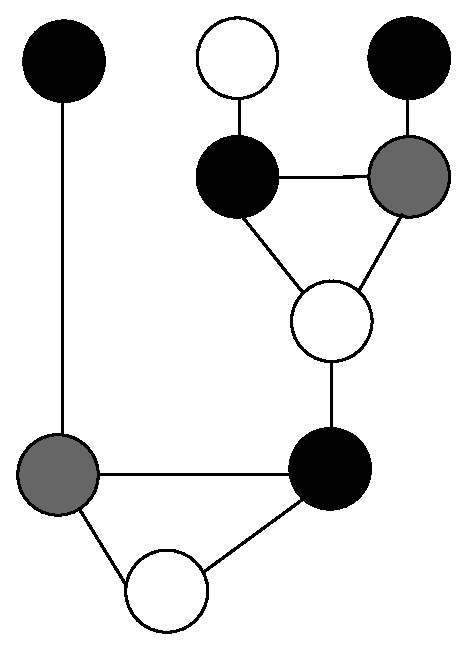
\includegraphics[width=0.1\textwidth]{informatika/teoreticka_informatika/obrazky/3COL1}

Kdy� do v��e uveden�ho konstruktu jakoby \uv{vlo��m} do horn� ��dky barvy, odpov�daj�c� t�� pravdivostn�m hodnot�m, nem��u spodn� vrchol obarvit jinak, ne� jako logick� or t�� barev. Tyto konstrukty mi budou slou�it pro reprezentaci $(a \vee b \vee c)$.

Ud�l�m si te� jeden st�edn� bod ($C$ jako centrum), k~n�mu p�id�m nejd��v dva body $T$ a $F$ a potom pro ka�dou prom�nnou p�id�m dva body, reprezentuj�c� $x$ a $\not x$ a spoj�m je dohromady a s~$C$. Ne� za�nu p�id�vat \uv{konstrukty} na vyhodnocov�n� trojic, pod�v�m se na vlastnosti. Mus� platit:

\begin{itemize}
\item $C$, $T$ a $F$ mus� m�t ka�d� jinou barvu
\item pro v�echny body mus� b�t bu� $x$ nebo $\not x$ $T$ barva a ta druh� $F$ barva
\end{itemize}

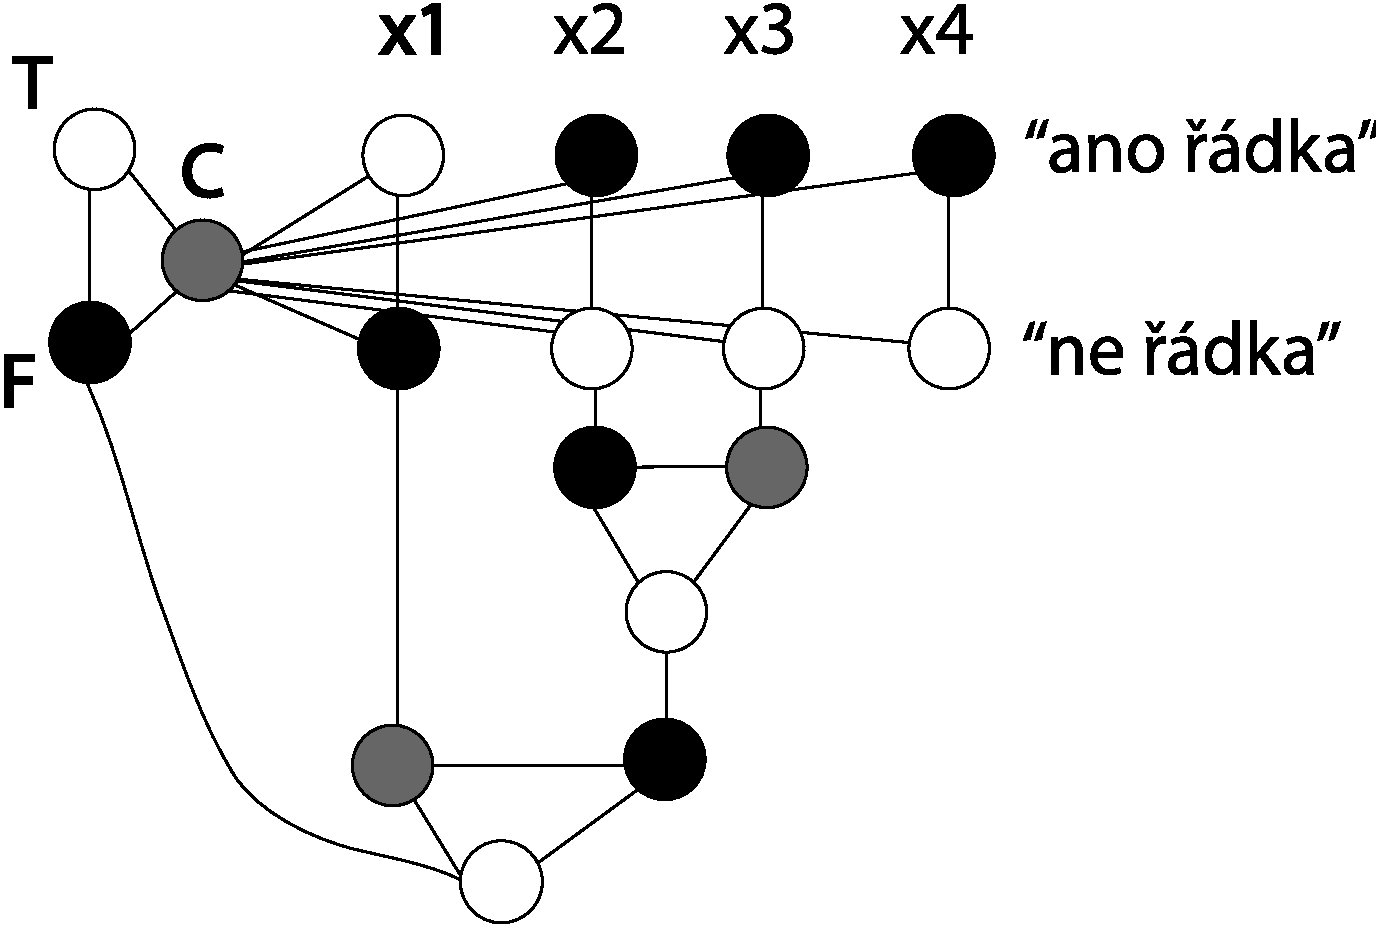
\includegraphics[width=0.8\textwidth]{informatika/teoreticka_informatika/obrazky/3COL2}

B�NO m��u ��ct, �e $C$ je �ediv�, $T$ b�l� a $F$ �ern�, �ern� mi vyjad�uje nepravdu, b�l� pravdu. Potom za n� \uv{nav�s�m} ty konstrukty -- bu� na $x$, nebo na $\not x$, podle toho, kter� z nich ve trojici zrovna je --  a jejich spodn� vrchol p�ipoj�m $F$�vrchol (to \uv{vynucuje}, aby vrchol byl $T$). Na obr�zku je formule $(\not x_1 \vee \not x_2 \vee \not x_3)$.

Tento graf je obarviteln� pr�v� tehdy, kdy� je formule splniteln�, a je sestaviteln� v~polynomi�ln�m �ase.

\end{e}
\end{e}

\begin{e}{Definice}{0}{t��da P}
 \textbf{T��du slo�itosti P} (n�kdy t� PTIME) tvo�� probl�my �e�iteln�
 sekven�n�mi deterministick�mi algoritmy v polynomi�ln�m �ase, tj. jejich �asov�
 slo�itost je $O(n^k)$. O algoritmech ve t��d� P tak� ��k�me, �e jsou
 \textbf{efektivn� �e�iteln�.}
\end{e}

\begin{e}{Definice}{0}{t��da NP}
 \textbf{T��da NP} (NPTIME) je t��da probl�m� �e�iteln�ch v polynomi�ln�m �ase
 sekven�n�mi nedeterministick�mi algoritmy. 
\end{e}

\begin{e}{Pozn�mka}{0}{0}
  V� se, �e $P \subseteq NP$. Nev� se v�ak, zda $P \neq NP$. P�edpokl�d� se to,
  ale je�t� to nikdo nedok�zal.
\end{e}

\begin{obecne}{P��klady probl�m� ze t��dy NP}
  \begin{pitemize}
    \item \textbf{KLIKA}(�pln� podgraf)~-- Je d�n neorientovan� graf $G$ a ��slo
    $k$. Existuje v $G$ �pln� podgraf velikosti aspo� $k$?
    \item \textbf{HK}(Hamiltonovsk� kru�nice)~-- Je d�n neorientovan� graf $G$.
    Existuje v $G$ Hamiltonovsk� kru�nice?
    \item \textbf{SP}(Sou�et podmno�iny)~-- Jsou d�na p�irozen� ��sla $a_1,
    \dots, a_n,b$. Existuje podmno�ina ��sel $a_1,\dots,a_n$, jej� sou�et je
    p�esn� $b$?
  \end{pitemize}
\end{obecne}

\begin{e}{Definice}{0}{NP-t�k� probl�m}
  Probl�m $B$ je \textbf{NP-t�k�}, pokud pro libovoln� probl�m $A$ ze t��dy NP
  plat�, �e $A$ je polynomi�ln� redukovateln� na $B$.
\end{e}

\begin{e}{Definice}{0}{NP-�pln� probl�m}
  Probl�m je \textbf{NP-�pln�}, pokud pat�� do t��dy NP a je NP-t�k�.
\end{e}

\begin{obecne}{D�sledky}
  \begin{pitemize}
    \item Pokud je $A$ NP-t�k� a nav�c je $A$ polynomi�ln� redukovateln� na $B$, tak je
      $B$ taky NP-t�k�.
    \item Pokud existuje polynomi�ln� algoritmus pro n�jak� NP-t�k� probl�m, pak
      existuj� polynomi�ln� algoritmy pro v�echny probl�my ve t��d� NP.
  \end{pitemize}
\end{obecne}

\begin{e}{V�ta}{0}{Cook-Levin 1971}
 Existuje NP-�pln� probl�m. (Dok�z�no pro SAT)
\end{e}

\subsection{Metoda rozd�l a panuj -- aplikace a anal�za slo�itosti}
Je to cel� napsan� dost rozvl��n�, ale podle m� nen� nutn� um�t cel� (nap��klad vzorce ze Strassena m��e cht�t jenom sadista), sp� tomu v�emu n�jak rozum�t. Zdroje: �epkovy a MJovy p�edn�ky na ADS1.
\\\\
\begin{definiceN}{Metoda rozd�l a panuj}
\emph{Rozd�l a panuj} je metoda n�vrhu algoritm� (ne strukturovan� programov�n�), kter� m� 3 kroky:
\begin{penumerate}
    \item \emph{rozd�l} -- rozd�l� �lohu na n�kolik pod�loh stejn�ho typu, ale men�� velikosti
    \item \emph{vy�e�} -- vy�e�� pod�lohy bu� p��mo pro dostate�n� mal� (�asto trivi�ln�), nebo rekurzivn� d�l�me d�l pokud jsou je�t� moc velk�
    \item \emph{sjedno�} -- sjednot� �e�en� pod�loh do �e�en� p�vodn� �lohy
\end{penumerate}
\end{definiceN}

\begin{poznamkaN}{Vytvo�en� rekurentn� rovnice}
Pro �asovou slo�itost algoritm� typu rozd�l a panuj zpravidla dost�v�m n�jakou rekurentn� rovnici.
\begin{pitemize}
    \item $T(n)$ budi� doba zpracov�n� �lohy velikosti $n$, za p�edpokladu, �e $T(n)=\Theta(1)$ pro $n\leq n_0$.
    \item $D(n)$ budi� doba na rozd�len� �lohy velikosti $n$ na $a$ pod�loh stejn� velikosti $\frac{n}{c}$. 
    \item $S(n)$ budi� doba na sjednocen� �e�en� pod�loh velikosti $\frac{n}{c}$ na jednu �lohu velikosti $n$.
\end{pitemize}
Dost�v�m rovnici
$$T(n)=\begin{cases} D(n)+aT(\frac{n}{c})+S(n) \quad\quad & n > n_0 \\ \Theta(1) & n \leq n_0 \end{cases}$$
\end{poznamkaN}

\subsubsection*{Metody �e�en� rekurentn�ch rovnic}

\begin{poznamkaN}{k �e�en� rekurentn�ch rovnic}
\begin{pitemize}
    \item P�edpoklad $T(n) = \Theta(1)$  pro dostate�n� mal� n nep�eme explicitn� do rovnice
    \item Zanedb�v�me celo��selnost (tj. p�eme $\frac{n}{2}$ m�sto $\lceil\frac{n}{2}\rceil$ a $\lfloor\frac{n}{2}\rfloor$)
    \item Nehled�me na konkr�tn� hodnoty aditivn�ch a multiplikativn�ch konstant, asymptotick� notace pou��v�m i v zad�n� rekurentn�ch rovnic, i v jejich �e�en�.
\end{pitemize}
\end{poznamkaN}


\begin{vetaN}{Substitu�n� metoda}
\begin{penumerate}
    \item Uhodnu asymptoticky spr�vn� �e�en�
    \item Indukc� ov���m spr�vnost (zvl�t� horn� a doln� odhad)
\end{penumerate}
\end{vetaN}

\begin{vetaN}{Metoda \uv{kucha�ka} (Master Theorem)}
Nech� $a\geq 1, c>1,d\geq 0\in\Real$ a nech� $T:\Nat\to\Nat$ je neklesaj�c� funkce takov�, �e $\forall n$ tvaru $c^k$ plat�
$$T(n)=aT(\frac{n}{c}) + \Theta(n^d)$$
Potom
\begin{penumerate}
    \item Je-li $a \neq c^d$, pak $T(n)$ je $\Theta( n^{\max\{\log_c a, d\}} )$
    \item Je-li $a = c^d$, pak $T(n)$ je $\Theta( n^d \log_c d )$
\end{penumerate}
\end{vetaN}

\begin{vetaN}{Master Theorem, varianta 2}
Nech� $0<a_i<1$, kde $i\in\{1,\dots,k\}$  a $d\geq 0$ jsou re�ln� ��sla a nech� $T:\Nat\to\Nat$ spl�uje rekurenci $$T(n)=\sum_{i=1}^k T(a_i\cdot n) + \Theta(n^d)$$ Nech� je ��slo $x$ �e�en�m rovnice $\sum_{i=1}^k a_i^x = 1$. Potom
\begin{penumerate}
    \item Je-li $x \neq d$ (tedy $\sum_{i=1}^k a_i^d \neq 1$), pak $T(n)$ je $\Theta( n^{\max\{x, d\}} )$
    \item Je-li $x = d$ (tedy $\sum_{i=1}^k a_i^d = 1$), pak $T(n)$ je $\Theta( n^d \log d )$
\end{penumerate}
\end{vetaN}

\subsubsection{N�soben� matic n$\times$n a Strassen�v algoritmus}

Nejd��ve si p�ipomeneme definici n�soben� dvou �tvercov�ch matic typu $n \times n$. Plat�, �e prvek v $i$-t�m ��dku a $j$-t�m sloupci v�sledn� matice $Z$ se rovn� standardn�mu skal�rn�mu sou�inu $i$-t�ho ��dku prvn� matice $X$ a $j$-t�ho sloupce druh� matice~$Y$. Form�ln� zaps�no:

$$ Z_{ij} = \sum_{k=1}^n X_{ik} \cdot Y_{kj}. $$

\begin{center}
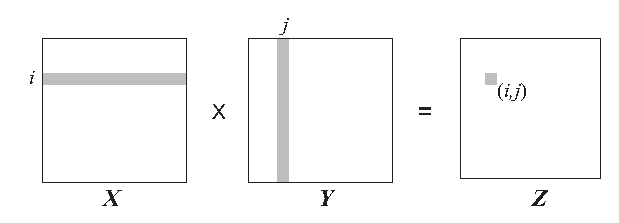
\includegraphics{informatika/algoritmy_a_ds/obrazky/nasobeni-matic.eps}
\end{center}
Algoritmus, kter� by n�sobil matice podle t�to definice, by m�l �asovou slo�itost $ \Theta(n^3) $, proto�e po�et prvk� ve v�sledn� matici je $n^2$ a jeden skal�rn� sou�in vektor� dimenze $n$ vy�aduje line�rn� po�et operac�.

My se s touto �asovou slo�itost� ov�em nespokoj�me a budeme postupovat podobn� jako p�i vylep�ov�n� algoritmu na n�soben� velk�ch ��sel. Bez �jmy na obecnosti p�edpokl�dejme, �e budeme n�sobit dv� matice typu $n \times n$, kde $n=2^k, k \in \bb N$. Ob� tyto matice rozd�l�me na �tvrtiny a tyto ��sti postupn� ozna��me u matice $X$ p�smeny $A$, $B$, $C$ a $D$, u matice $Y$ p�smeny $P$, $Q$, $R$ a $S$. Z definice n�soben� matic zjist�me, �e �tvrtiny v�sledn� matice $Z$ m��eme zapsat pomoc� sou�in� ��st� n�soben�ch matic. Lev� horn� �tvrtina bude odpov�dat v�sledku operac� $AP+BR$, prav� horn� �tvrtina bude $AQ+BS$, lev� doln� $CP+DR$ a zbyl� $CQ+DS$ (viz obr�zek).

\begin{center}
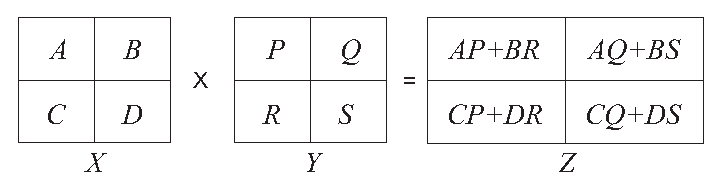
\includegraphics{informatika/algoritmy_a_ds/obrazky/nasobeni-matic-2.eps}
\\{N�soben� roz�tvrcen�ch matic}
\end{center}


P�evedli jsme tedy probl�m n�soben� �tvercov�ch matic ��du $n$ na n�soben� �tvercov�ch matic ��du ${n/2}$. T�mto rozd�lov�n�m bychom mohli pokra�ovat, dokud bychom se nedostali na matice ��du 1, jejich� vyn�soben� je trivi�ln�. Dostali jsme tedy klasick� algoritmus typu {\it rozd�l a panuj}. Pomohli jsme si ale n�jak? V ka�d�m kroku prov�d�me 8 n�soben� matic polovi�n�ho ��du a nav�c konstantn� po�et operac� na $n^2$ prvc�ch. Dost�v�me tedy rekurentn� z�pis �asov� slo�itosti:

$$ T(n) = 8T\left({n \over 2}\right) + \Theta(n^2). $$

Pou�it�m Master Theoremu lehce dojdeme k z�v�ru, �e slo�itost je st�le $\Theta(n^3)$, tedy stejn� jako p�i n�soben� matic z definice. Zd�nliv� jsme si tedy nepomohli, ale stejn� jako tomu bylo u n�soben� velk�ch ��sel, i te� m��eme zredukovat po�et n�soben� matic polovi�n�ho ��du, kter� nejv�ce ovliv�uje �asovou slo�itost algoritmu. Nen� to bohu�el nic trivi�ln�ho, a proto si rad�ji rovnou �ekneme spr�vn� �e�en�. Jedn� se o Strassen�v algoritmus, kter� redukuje pot�ebn� po�et n�soben� na~7, a je�t� p�ed t�m, ne� si uk�eme, jak funguje, dok�eme si, jak n�m to s �asovou slo�itost� vlastn� pom��e:

$$ T(n) = 7T\left({n \over 2}\right) + \Theta(n^2) \Longrightarrow \Theta(n^{\log_2 7}) = \Theta(n^{2.808}). $$

V�sledn� slo�itost Strassenova algoritmu je tedy $\Theta(n^{2.808})$, co� je sice mal�, ale pro velk� matice znateln� zlep�en� oproti algoritmu vych�zej�c�mu p��mo z~definice \footnote{
Zat�m nejlep�� dok�zan� algoritmus m� �asovou slo�itost $\Theta(n^{2.376})$, $ $ ov�em s velkou multiplikativn� konstantou.} \footnote{Strassen se da pouzit i pro vypocet determinantu.}.
\\\\
\begin{lemmaN}{vzorce pro n�soben� blokov�ch matic ve~Strassenov� algoritmu}

\def\\{\noalign{\vskip 7pt}}

$$
\begin{pmatrix}A & B \\ C & D \end{pmatrix}
\cdot
\begin{pmatrix}P & Q \\ R & S \end{pmatrix}
=
\begin{pmatrix}
T_1 + T_4 - T_5 + T_7 &
T_3 + T_5 \\
T_2 + T_4 &
T_1 - T_2 + T_3 + T_6
\end{pmatrix}$$

kde:

$$\vbox{\halign{$#$\hfil\qquad &$#$\hfil\qquad \cr
T_1 = (A+D)\cdot(P+S)           & T_5 = (A+B)\cdot S \cr\\
T_2 = (C+D)\cdot P              & T_6 = (C-A)\cdot (P+Q) \cr\\
T_3 = A\cdot(Q-S)               & T_7 = (B-D)\cdot (R+S) \cr\\
T_4 = D\cdot(R-P)                                        \cr
}}$$
\end{lemmaN}
% \proof Do �tverc� $4 \times 4$ si nap�eme znaky $+$ nebo $-$ podle toho, jestli se p�i v�po�tu dan� matice p�i��t� nebo ode��t� p��slu�n� sou�in dvou matic. ��dky znamenaj� matice $A$, $B$, $C$ a $D$ a sloupce zna�� matice $P$, $Q$, $R$ a $S$. Pokud se tedy v prvn�m ��dku a prvn�m sloupci vyskytuje znak $+$, znamen� to �e p�i�teme sou�in matic $A$~a~$P$. Nejd��ve si spo��t�me pomocn� matice $T_1$ a� $T_7$ a z nich pak dopo��t�me, co bude na p��slu�n�ch m�stech ve v�sledn� matici.
% 
% $$
% T_1 = \begin{pmatrix}+&.&.&+\\.&.&.&.\\.&.&.&.\\+&.&.&+\end{pmatrix} \qquad
% T_2 = \begin{pmatrix}.&.&.&.\\.&.&.&.\\+&.&.&.\\+&.&.&.\end{pmatrix} \qquad
% T_3 = \begin{pmatrix}.&+&.&-\\.&.&.&.\\.&.&.&.\\.&.&.&.\end{pmatrix} \qquad
% T_4 = \begin{pmatrix}.&.&.&.\\.&.&.&.\\.&.&.&.\\-&.&+&.\end{pmatrix}
% $$
% $$
% T_5 = \begin{pmatrix}.&.&.&+\\.&.&.&+\\.&.&.&.\\.&.&.&.\end{pmatrix} \qquad
% T_6 = \begin{pmatrix}-&-&.&.\\.&.&.&.\\+&+&.&.\\.&.&.&.\end{pmatrix} \qquad
% T_7 = \begin{pmatrix}.&.&.&.\\.&.&+&+\\.&.&.&.\\.&.&-&-\end{pmatrix}\qquad
% $$
% 
% \medskip
% 
% \def\\{\noalign{\vskip 7pt}}
% $$
% T_1 + T_4 - T_5 + T_7 &= \begin{pmatrix}+&.&.&.\\.&.&+&.\\.&.&.&.\\.&.&.&.\end{pmatrix} = AP + BR \\
% T_3 + T_5 &= \begin{pmatrix}.&+&.&.\\.&.&.&+\\.&.&.&.\\.&.&.&.\end{pmatrix} = AQ + BS \\
% T_2 + T_4 &= \begin{pmatrix}.&.&.&.\\.&.&.&.\\+&.&.&.\\.&.&+&.\end{pmatrix} = CP + DR \cr\\
% T_1 - T_2 + T_3 + T_6 &= \begin{pmatrix}.&.&.&.\\.&.&.&.\\.&+&.&.\\.&.&.&+\end{pmatrix} = CQ + DS
% $$
% \\\\
% % konec slidu z prednasky

% Jak je vid�t, v�sledn� matice je tvo�ena stejn�mi ��stmi jako p�i oby�ejn�m n�soben�. 

\\\\
\subsubsection{Hled�n� medi�nu v lin. �ase (Blum et al.)}
\begin{algoritmusN}{Blum et al.}
\emph{Select(X,k)}
\begin{penumerate}
\item Pokud $n \leq 5 \Rightarrow$ vy�e��me p��mo
\item Vstup rozd�l�me na p�tice $P_1 . . . P_{\lceil n/5\rceil}$ (posledn� m��e b�t ne�pln�), to zvl�dneme v $O(n)$
\item  $\forall i\in\{1...\lceil n/5\rceil\}:~~ m_i := median(Pi)$, to zvl�dneme v $O(n)$
\item $ pivot := Select (m_1,...,m_{\lceil n/5\rceil}, \lceil n/10\rceil)$     (medi�n medi�n�)
\item Rozd�lime X na L(=men�� ne� pivot), S(=stejn� jako pivot), P(=v�t�� ne� pivot)
\item Rekurzivn� se zavolame na jednu z L, S, P (tu, ve ktere se ma vyskytovat hledany prvek � zjist�me podle jejich velikosti)
\end{penumerate}
\end{algoritmus}
\begin{obecne}{�asov� slo�itost:} V ka�d�m kroku vypadne alespo� $\frac{3n}{10}$ prvk�.
\proof P�edstavme si vybran� p�tice se�azen� podle velikosti od nejv�t��ho prvku a zakresleme je do sloupc�. Jejich medi�ny tedy vypl�uj� prost�edn� �adu. Tyto p�tice pak se�a�me podle velikosti jejich medi�n� (nejmen�� vlevo). Hledan� pivot se tedy nach�z� (pokud p�edpokl�d�me pro jednoduchost lich� po�et p�tic) p�esn� uprost�ed. O prvc�ch nad pivotem a napravo od n�j m��eme ur�it� ��ct, �e jsou v�t�� nebo rovny pivotu, prvky pod n�m a nalevo od n�j jsou zase ur�it� men�� nebo rovny pivotu. Podle algoritmu v�dy vypadne jedna nebo druh� skupina prvk� o velikosti alespo� $\frac{3n}{10}$ prvk� (z obr�zku).
\begin{center}
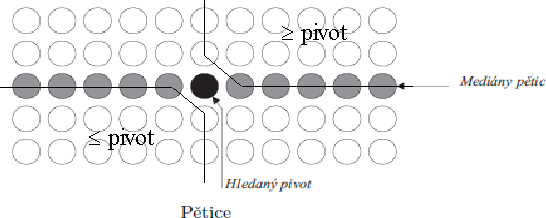
\includegraphics[scale=1.8]{informatika/algoritmy_a_ds/obrazky/petice.png}
\end{center}
V ka�d�m kroku funkce vol� sama sebe na vstup velikosti nejv��e n/5 a pak na 7n/10 ostatn� operace jsou line�rn�, nejhor�� p��pad: $T(n)=O(n)+T(\frac{n}{5})+T(\frac{7n}{10}) $, odhadneme �e odpov�d� lin.slo�itosti O(n).
\proof
Indukc� �e $T(n) = O(n):\exists k>0 \exists n_0 \forall n>n_0: T(n)\leq kn $ pro n�jakou dostate�n� velkou konstantu k.
\begin{penumerate}
\item $n=1: T(n)= 1+k\frac{9}{10}\leq  k1$
\item $T(n)=O(n)+T(\frac{n}{5})+T(\frac{7n}{10})\leq n + k\frac{n}{5} + k\frac{7n}{10} = n + k\frac{9n}{10}$
\\
$n + k\frac{9n}{10} \leq kn \Rightarrow n \leq \frac{1}{10}kn \Rightarrow 10 \leq k$
\end{penumerate}


\subsubsection{MergeSort}

Tento t��d�c� algoritmus pracuje na~principu, �e vstup rozd�l�me na~dv� (skoro) stejn� velk� ��sti, kter� rekurzivn�m vol�n�m set��d�me, a~nakonec v�sledn� dv� posloupnosti slijeme do~jedn�. 

\begin{algoritmusN}{MergeSort}

\begin{penumerate}
\item Vstup: posloupnost $x_1,\dots, x_n$.
\item Pokud $n \leq 1 \Rightarrow$ vr�t�me vstup.
\item $y_1,\dots,y_{\lfloor n/2 \rfloor} \leftarrow$ \emph{MergeSort} $(x_1,\dots,x_{\lfloor n/2 \rfloor})$.
\item $z_1,\dots,z_{\lceil n/2 \rceil} \leftarrow$ \emph{MergeSort} $(x_{\lfloor n/2 \rfloor + 1},\dots,x_n)$.
\item Vr�t�me \emph{MergeSort} $(y_1,\dots,y_{\lfloor n/2 \rfloor}; z_1,\dots,z_{\lceil n/2 \rceil})$.
\end{penumerate}

\noindent
Na slit� dvou set��d�n�ch posloupnost� do~jedn� pou��v�me funkci Merge:
\\\noindent
\emph{Merge} $(y_1, \dots,y_a;z_1, \dots,z_b)$

\begin{penumerate}
\item $i \leftarrow 1, j \leftarrow 1, k \leftarrow 1$.
\item Dokud $k \leq a+b$:
\item ~~~~~~~~Je-li $(j>b)$ nebo $(i \leq a) \& (y_i < z_j) \Rightarrow x_k \leftarrow y_i, k++, i++$.
\item ~~~~~~~~Jinak $\Rightarrow x_k \leftarrow z_j, k++, j++$.
\item Vr�t�me $x_1, \dots,x_n$.
\end{penumerate}

\s{Pozorov�n�:}
\emph{Merge} trv� $\Theta (n)$, nebo� ka�dou ze~sl�van�ch posloupnost� projdeme pr�v� jednou.

\medskip

\begin{obecne}{�asov� slo�itost:}

Rozd�lov�n� a~sl�v�n� n�m trv� line�rn� dlouho, tak�e pro �asovou slo�itost MergeSortu plat� tato rekurentn� rovnice, kterou vyresime pomoc� MT: $$T(n)= 2 \cdot T(n/2) + \Theta(n)  \Longrightarrow \Theta(n^1\log n}) = \Theta(n\log n).$$ 
\end{obecne}

\begin{obecne}{Pam�ov� slo�itost:}

$$M(n) = d \cdot n + M(n/2) = d \cdot n + d \cdot n/2 + d \cdot n/4 + \dots \leq 2d n = \Theta(n).$$

Tento vztah plat� pro n�jakou vhodnou konstantu $d$. M��eme ho op�t nahl�dnout nap��klad ze stromu rekurzivn�ch vol�n�. Pod�vejme se na~libovolnou cestu od~ko�ene do~listu. V~jednotliv�ch vrcholech pot�ebujeme pam�ti p�esn� $d \cdot n/2^k$, kde $k$ je ��slo hladiny. Kdy� tyto hodnoty se�teme p�es v�echny vrcholy na~t�to cest�, v�sledek bude konvergovat k~$2dn$, co� d�v� pam�ovou slo�itost $\Theta(n)$.
\end{obecne}
\begin{obecne}{Z�v�r:}
Mergesort b�� V~�ase $\Theta(n \log{n})$ a~pam�ti $\Theta(n)$. Line�rn� pam�ov� slo�itost nen� v�hodn�, ale na~druhou stranu se tento algoritmus velmi hod� nap��klad na~t��d�n� line�rn�ch spojov�ch seznam�.

\def\b#1{\mathbf{#1}}


\subsection{Bin�rn� vyhled�vac� stromy, vyva�ov�n�, haldy}

\subsubsection*{Bin�rn� strom}

\begin{e}{Definice}{0}{0}
\emph{Dynamick� mno�ina} je mno�ina prvk� (datov� struktura), m�n�c� se v �ase. Ka�d� jej� prvek je p��stupn� p�es ukazatel a obsahuje:
\begin{pitemize}
    \item \emph{kl��} (jednu polo�ku, typicky hodnotu z lin. uspo��dan� mno�iny), 
    \item \emph{ukazatel(e)} na dal�� prvky, 
    \item p��padn� \emph{dal�� data}.
\end{pitemize}
Na takov� mno�in� jsou definov�ny tyto operace:
\begin{pitemize}
    \item \emph{find} - nalezen� prvku podle kl��e
    \item \emph{insert} - p�id�n� dal��ho prvku
    \item \emph{delete} - odstran�n� prvku
    \item \emph{min}, \emph{max} - nalezen� nejv�t��ho / nejmen��ho prvku
    \item \emph{succ}, \emph{pred} - nalezen� n�sleduj�c�ho / p�edch�zej�c�ho prvku k n�jak�mu p�edem dan�mu
\end{pitemize}
\end{e}


\begin{e}{Definice}{0}{0}
\emph{Bin�rn� strom} je dynamick� mno�ina, kde ka�d� prvek (uzel, node) m� krom� kl��e a p��p. dal��ch dat t�i ukazatele na \emph{lev�ho} a \emph{prav�ho} syna a rodi�e. Speci�ln� uzel je \emph{ko�en}, kter� m� NULLov� ukazatel na rodi�e. Ten je v bin�rn�m strom� jeden. Uzly, kter� maj� NULLov� ukazatele na prav�ho i lev�ho syna, se naz�vaj� \emph{listy}.

\emph{Podstrom} je ��st stromu (vybran� prvky), kter� je sama stromem - nap�. pokud se jako ko�en ur�� jeden z prvk�. \emph{Lev�(prav�)} podstrom n�jak�ho prvku je strom, ve kter�m je ko�enem lev�(prav�) syn tohoto prvku. \emph{V��ka stromu} je d�lka nejdel�� cesty od ko�enu k listu.
\end{e}

Bin�rn� strom je \emph{vyv�en�}, pokud max. 1 uzel m� jednoho syna (tj. v�echny vnit�n� uzly krom� a� na jeden maj� oba syny, listy z definice nemaj� ��dn�ho). V��ka vyv�en�ho stromu roste logaritmicky vzhledem k po�tu uzl�. V��ka nevyv�en�ho stromu m��e r�st a� line�rn� vzhledem k po�tu prvk� (i \uv{spojov� seznam} je platn� bin. strom).


\subsubsection*{Bin�rn� vyhled�vac� strom}

\begin{e}{Definice}{0}{0}
\emph{Bin�rn� vyhled�vac� strom} je takov� bin�rn� strom, ve kter�m je jeho struktura ur�en� podle kl��u jeho uzl�: pro ka�d� uzel s kl��em hodnoty $k$ plat�, �e jeho lev� podstrom obsahuje jen uzly s men�� hodnotou kl��e ne� $k$ a jeho prav� podstrom jen uzly s hodnotou kl��e v�t�� nebo rovnou $k$.
\end{e}

\begin{e}{Algoritmus}{0}{Vyhled�v�n� v bin. strom�}
\begin{verbatim}
Find( x - ko�en, k - hledan� hodnota kl��e ){
  while( x != NULL && k != x->kl�� ){
    if ( k < x->kl�� )
      x = x->lev�_syn;
    else
      x = x->prav�_syn;
  }
  return x;
}
\end{verbatim}

Slo�itost je $O(h)$ v nejhor��m p��pad�, kde $h$ je v��ka stromu (tj. pro nevyv�en� stromy a� $O(n)$ kde $n$ je po�et prvk�). Asymptotick� �asov� slo�itost ostatn�ch operac� je stejn�.

Vlo�en� a vymaz�n� prvku se prov�d� prost�m nalezen�m m�sta, kam by se prvek m�l vlo�it (nebo kde u� je), a p�epojen�m pointer�.
\end{e}

\subsubsection*{Vyva�ovan� vyhled�vac� stromy}

Kv�li zaji�t�n� v�t�� rychlosti (men�� asymptotick� �asov� slo�itosti) operac� byly vytvo�eny speci�ln� druhy bin�rn�ch vyhled�vac�ch strom�, kter� jsou pr�b�n� vyva�ov�ny, aby m�ly max. v��ku men�� ne� $c\cdot\log n$, kde $n$ je po�et uzl� a $c$ n�jak� konstanta.

\begin{e}{Definice}{0}{Pomocn� operace na stromech}
Pro vyva�ov�n� strom� p�i vkl�d�n� a odeb�r�n� uzl� se definuj� pomocn� operace: \emph{prav�} a \emph{lev� rotace}. Zachov�vaj� vlastnosti bin. vyhled�vac�ch strom� a jsou provediteln� v konstatn�m �ase - jde jen o p�epojen� uzl� n�sl. zp�sobem (pro pravou rotaci na uzlu $Q$ a levou na $P$):

\begin{center}
\includegraphics[width=12cm]{informatika/algoritmy_a_ds/obrazky/tree_rotation.png}

(Zdroj obr�zku: Wikipedia)
\end{center}
\end{e}


\begin{e}{Definice}{0}{�erveno-�ern� stromy}
�erveno-�ern� stromy jsou bin�rn� vyhled�vac� stromy s garantovanou max. v��kou $O(\log n)$, kde $n$ je po�et uzl�, tj. operace na nich mohou m�t asymptotickou �asovou slo�itost $O(\log n)$. Pro jejich popis je nutn� definovat \emph{intern� uzly} - v�echny uzly stromu a \emph{extern� uzly} - na (intern�ch) listech (a uzlech s jedn�m potomkem) um�le p�idan� NULLov� ukazatele (de facto \uv{listy} �erveno-�ern�ho stromu). Extern� uzly slou�� jenom jako abstrakce pro popis strom�, p�i implementaci se s nimi neoperuje. �erveno-�ern� strom m� tyto �ty�i povinn� vlastnosti:
\begin{penumerate}
    \item Ka�d� uzel (extern� i intern�) m� definovanou barvu, a to �ernou nebo �ervenou.
    \item Ka�d� extern� uzel je �ern�.
    \item Ka�d� �erven� vrchol mus� m�t oba syny �ern�.
    \item Ka�d� cesta od libovoln�ho vrcholu k list�m v jeho podstrom� mus� obsahovat stejn� po�et �ern�ch uzl�.
\end{penumerate}

Pro �erveno-�ern� stromy se definuje \emph{v��ka uzlu} $x$ ($\b{h}(x)$) jako po�et uzl� na nedel�� mo�n� cest� k listu v jeho podstrom�. \emph{�ern� v��ka uzlu} ($\b{bh}(x)$) je po�et �ern�ch uzl� na takov� cest�.
\end{e}

\begin{e}{V�ta}{0}{Vlastnosti �erveno-�ern�ch strom�}
Podstrom libovoln�ho uzlu $x$ obsahuje alespo� $2^{\b{bh}(x)}-1$ intern�ch uzl�. D�ky tomu m� �erveno-�ern� strom v��ku v�dy nejv��e $2\log(n+1)$ (kde $n$ je po�et uzl�). (D�kaz prvn�ho tvrzen� indukc� podle $\b{h}(x)$, druh�ho z prvn�ho a t�et� vlastnosti �erveno-�ern�ch strom�)
    \end{e}

\begin{e}{D�sledek}{0}{0}
Operace hled�n� (minima, maxima, n�sledn�ka, \dots), kter� jsou stejn� jako u obecn�ch bin�rn�ch vyhled�vac�ch strom�, maj� garantovanou �asovou slo�itost $O(\log n)$.
\end{e}

\begin{e}{Algoritmus}{0}{Vkl�d�n� a odeb�r�n� uzl� v �erveno �ern�ch stromech}
Ob� operace maj� podle garantovan� max. v��ky garantovanou �as. slo�itost $O(\log n)$ pro $n$ po�et uzl�. Proto�e bez poru�en� vlastnost� �erveno-�ern�ch strom� lze ko�en v�dy p�ebarvit na�erno, m��eme pro n� p�edpokl�dat, �e \emph{ko�en stromu} je \emph{v�dy �ern�}.

\emph{Vkl�d�n�} vypad� n�sledovn�:
\begin{pitemize}
    \item Nalezen� m�sta pro vlo�en� a p�id�n� nov�ho prvku jako v obecn�ch bin. vyhl. stromech, nov� prvek se p�ebarv� na�erveno.
    \item Pokud je jeho otec �ern�, m��eme skon�it -- vlastnosti strom� jsou spln�n�. Pokud je �erven�, mus�me strom upravovat (tady p�edpokl�d�m, �e otec p�id�van�ho uzlu je lev�m synem, opa�n� p�ipad je symetrick�):
    \item Je-li i str�c �erven�, p�ebarvit otce a str�ce na�erno a p�en�st chybu o patro v�� (je-li d�d �ern�, kon��m, jinak m��u pokra�ovat a� do ko�ene, kter� u� lze p�ebarvovat beztrestn�).
    \item Je-li str�c �ern� a p�idan� uzel je lev�m synem, ud�lat pravou rotaci na d�dovi a p�ebarvit uzly tak, aby odpov�daly vlastnostem strom�.
    \item Je-li str�c �ern� a p�idan� uzel je prav�m synem, ud�lat levou rotaci na otci a p�ev�st tak na p�edchoz� p��pad.
\end{pitemize}

\emph{Odeb�r�n�} se prov�d� takto:
\begin{pitemize}
    \item Odstran�m uzel stejn� jako v p�edchoz�m p��pad�. Opravdu odstran�n� uzel (z p�epojov�n�) m� max. jednoho syna. Pokud odstra�ovan� uzel byl �erven�, neporu��m vlastnosti strom�, stejn� tak pokud jeho syn byl �erven� -- to �e��m jeho p�ebarven�m na�erno.
    \item V opa�n�m p��pad� (tj. syn odeb�ran�ho -- $x$ -- je �ern�) mus�m ud�lat n�sl. �pravy (p�ep. �e $x$ je lev�m synem sv�ho nov�ho otce, v op. p��pad� postupuji symetricky):
    \item $x$ prohl�s�m za \uv{dvojit� �ern�} a t�to vlastnosti se pokou��m zbavit.
    \item Pokud je bratr $x$ (bu� $w$) �erven�, pak m� 2 �ern� syny -- provedu levou rotaci na rodi�i $x$, prohod�m barvy rodi�e $x$ a uzlu $w$ a p�evedu tak situaci na jeden z n�sl. p��pad�:
    \item Je-li $w$ �ern� a m�-li 2 �ern� syny, prohl�s�m $x$ za �ern� a p�ebarv�m $w$ na�erveno, rodi�e p�ebarv�m bu� na �erno (a kon��m) nebo na \uv{dvojit� �ernou} a propaguji chybu (mohu doj�t a� do ko�ene, kter� lze p�ebarovat beztrestn�).
    \item Je-li $w$ �ern�, jeho lev� syn �erven� a prav� �ern�, vym�n�m barvy $w$ s jeho lev�m synem a na $w$ pou�iji pravou rotaci, ��m� dostanu posledn� p��pad:
    \item Je-li $w$ �ern� a jeho prav� syn �erven�, p�ebarv�m prav�ho syna na�erno, odstran�m dvojit� �ernou z $x$, provedu levou rotaci na $w$ a pokud m�l p�vodn� $w$ (a $x$) �erven�ho otce, p�ebarv�m $w$ na�erveno a tohoto (te� u� lev�ho syna $w$) p�ebarv�m na�erno.
\end{pitemize}
\end{e}


\begin{e}{Definice}{0}{AVL stromy (Adelson-Velsky \& Landis)}
\emph{AVL stromy} jsou, podobn� jako �erveno-�ern� stromy, bin. vyhled�vac� stromy, kter� zaru�uj� max. logaritmick� n�r�st v��ky vzhledem k po�tu prvk�. Pro ka�d� uzel $x$ se v AVL stromu definuje \emph{faktor vyv�en�} jako rozd�l v��ky jeho lev�ho a prav�ho podstromu: $\b{bf}(x) = h(\texttt{x->lev�}) - h(\texttt{x->prav�})$. Pro v�echny uzly v AVL stromu plat�, �e $|\b{bf}(x)|\leq 1$.
\end{e}

\begin{e}{V�ta}{0}{Zaru�en� v��ky AVL strom�}
V��ka AVL stromu s $n$ vrcholy je $O(\log n)$. (D�kaz: bu� $T_n$ AVL strom v��ky $n$ s minim�ln�m po�tem uzl�. Ten m� podstromy $T_{n-1}$ a $T_{n-2}$ atd., tj. velikost minim�ln�ho AVL stromu roste jako Fibonacciho posloupnost, tedy $|T_n|\geq (\frac{1+\sqrt{5}}{2})^{n-1}$. D�kaz tohoto indukc�.)
\end{e}

\begin{e}{Algoritmus}{0}{Operace na AVL stromech}
Vyhled�vac� operace se prov�d� stejn� jako na obecn�ch bin. vyhled�vac�ch stromech, vkl�d�n� a odeb�r�n� prvk� taky, ale pokud tyto operace poru�� z�kl. vlastnost AVL strom� ($|\b{bf}(x)=2|$), je nutn� prov�st vyva�ov�n� -- pomoc� rotac� (kter� mohou b�t propagov�ny a� ke ko�eni). P�i vkl�d�n� a odeb�r�n� je nav�c nutn� pr�b�n� (nejh��e a� ke ko�eni) upravovat indikaci faktoru vyv�en� jednotliv�ch uzl�.
\end{e}

\subsubsection*{Halda}

\begin{e}{Definice}{0}{0}
\emph{Halda(heap)} je dynamick� mno�ina se stromovou strukturou (bin�rn� halda je bin�rn� strom), pro kterou plat� tzv. \uv{vlastnost haldy}: $$\text{ Je-li }x\text{ potomek }y\text{, pak }x\texttt{->kl��}\geq y\texttt{->kl��}$$ Haldy s touto nerovnost� jsou tzv. \emph{min-heap}y, pokud je nerovnost opa�n�, jde o \emph{max-heap}.
\end{e}

\begin{obecne}{(Bin�rn�) haldy}
Bin�rn� haldy jsou nej�ast�j��m typem haldy. Zaji��uj� nalezen� minim�ln�ho prvku v konstantn�m �ase a odebr�n� a p�id�n� minima v �ase $O(\log n)$. V ka�d� hladin� od prvn� a� do p�edposledn� je max. mo�n� po�et uzl�, v posledn� jsou uzly co nejv�ce \uv{vlevo} -- tedy max. v��ka haldy s $n$ prvky je $(\log n) + 1$. Proto je pro bin�rn� haldy jednodu�e provediteln� jejich datov� reprezentace polem (bez pointer�), kde p�i indexov�n� od 0 m� uzel na indexu $k$:
\begin{pitemize}
    \item Lev�ho a prav�ho syna na indexu $2k+1$, resp. $2k+2$ (pokud to nen� v�c ne� celk. po�et prvk�, potom syny nem�).
    \item Rodi�e na indexu $\lceil\frac{k}{2}\rceil-1$. 
\end{pitemize}

\emph{P�id�n� uzlu} do haldy znamen� p�id�n� prvku na konec haldy a dokud m� jeho rodi� v�t�� kl��, jeho prohazov�n� s rodi�em (tedy posouv�n� o vrstvu v��). P�i \emph{odeb�r�n� uzlu} z haldy tento nahrad�m posledn�m prvkem v hald� a potom dokud neplat� vlastnost haldy (nejm�n� jeden z potomk� m� men�� kl��), prohazuji ho s potomkem s men��m kl��em (a posouv�m o vrstvu n�).

Vytvo�en� haldy je mo�n� v �ase $O(n)$, kde $n$ je po�et prvk� v hald� -- p�id�n� 1 prvku do haldy trv� $O(h)$, kde $h$ je aktu�ln� v��ka (a $h$ roste od $0$ a� k $\lceil\log n\rceil$, po�et prvk� ve v��ce $k$ je $\frac{n}{2^{k+1}}$, bereme-li v��ku list� rovnou nule) - v sou�tu za v�echny prvky jde o $O(n\cdot\sum_{h=0}^{\lceil\log n\rceil}\frac{h}{2^h})$.

Bin�rn� halda se pou��v� nap�. k \emph{t��d�n� haldou} (heapsortu), kdy se z dat, kter� je pot�eba ut��dit, nejd��ve postav� halda, a potom se opakuje operace odebr�n� ko�ene (tj. minim�ln�ho prvku).
\end{obecne}

\begin{obecne}{Fibonacciho haldy}
Fibonacciho haldy maj� n�zkou �asovou slo�itost b�n�ch operac� -- amortizovan� $O(1)$ pro vlo�en�, hled�n� minima apod.; odebr�n� prvku a odebr�n� minima m� slo�itost $O(\log n)$ pro $n$ prvk� v hald�. Tvo�� ji skupina strom�, vyhovuj�c�ch \uv{vlastnosti haldy}. Ka�d� uzel haldy s $n$ prvky m� max. $\log n$ potomk� a ve sv�m podstrom� minim�ln� $F_{k+2}$ uzl�, kde $F_k$ je $k$-t� Fibonacciho ��slo. To je zaji�t�no pravidlem, �e p�i odeb�r�n� prvk� lze z neko�enov�ho uzlu odd�lit max. 1 syna, jinak je nutn� odd�lit i tento uzel a ten se pak stane ko�enem dal��ho stromu. Po�et strom� se sni�uje p�i odeb�r�n� minima, kdy jsou spojov�ny dohromady.

Fibonacciho haldy se pou��vaj� pro efektivn� implementaci slo�it�j��ch operac�, jako nap�. Jarn�kova nebo Dijkstrova algoritmu.
\end{obecne}

\newcommand{\nadpis}[1]{\pagebreak[2]\ramcek{\subsubsection*{#1}}}

\subsection{Hašování}

\begin{definiceN}{slovníkový problém} Dáno univerzum $U$, máme reprezentovat
$S \subseteq U$ a navrhnout algoritmy pro operace
\begin{pitemize}
\item MEMBER(x) - zjistí zda $x \in S$ a pokud ano nalezne kde,
\item INSERT(x) - pokud $x \notin S$, vloží $x$ do struktury reprezentující $S$,
\item DELETE(x) - když $x \in S$, smaže $x$ ze struktury reprezentující $S$.
\end{pitemize}
\end{definiceN}

Například pomocí pole můžeme tyto operace implementovat rychle, ale nevýhodou
je prostorová náročnost. Pro velké množiny je to někdy dokonce nemožné.
\emph{Hašování} se snaží zachovat rychlost operací a odstranit prostorovou
náročnost.

Podívejme se nyní na \emph{základní ideu} hašování. Mějme univerzum $U$ a
množinu $S \subseteq U$ takovou, že $|S| << |U|$. Dále mějme funkci
$h:U\rightarrow\{0,1,\dots,m-1\}$. Množinu $S$ potom reprezentujeme tabulkou
(polem) o velikosti $m$ tak, že prvek $x \in S$ je uložen na řádku $h(x)$.

\begin{definiceN}{Hašovací funkce, kolize} Funkci
$h:U\rightarrow\{0,1,\dots,m-1\}$ potom nazýváme \textbf{hašovací funkcí}.
Situaci $h(s)=h(t)$, pro $s \neq t; s,t \in S$  nazveme \textbf{kolize}.
\end{definiceN}

Jelikož mohutnost univerza $U$ je větší než velikost hašovací tabulky, nelze se
kolizím úplně vyhnout. Existuje spousta různých metod, jak kolize řešit.
Podívejme se tedy na některé podrobněji.

\begin{definice}
Ještě si zavedeme některé značení. Velikost $S$ (hašované množiny) označme
\textbf{n}, velikost tabulky (pole) označme \textbf{m}, a faktor naplnění
\textbf{$\alpha=\frac{n}{m}$}.
\end{definice}

\subsubsection*{Hašování se separovanými řetězci}

Použijeme pole velikosti $m$, jehož $i$-tá položka bude spojový seznam $S_i$
takový, že $s\in S_i \Leftrightarrow h(s)=i$, pro $s\in S$. Čili každý řádek
pole obsahuje spojový seznam všech (kolidujících) prvků, které jsou hašovány na
tento řádek. Seznamy nemusí být uspořádané, vznikají tak, jak jsou vkládány
jednotlivé prvky do struktury.

\begin{algoritmusN}{Hašování se separovanými řetězci}
\begin{pitemize}
\item \textbf{MEMBER} -- Spočteme hodnotu hašovací funkce $h(x)$, prohledáme
řetězec začínající na pozici $h(x)$ a zjistíme zda se prvek nachází, či
nenachází ve struktuře. Pokud se prvek v databázi nachází, tak musí nutně ležet
v tomto řetězci.
\item \textbf{INSERT} -- Zjistíme zda $x$ je v řetězci $h(x)$, pokud ne, přidáme
ho nakonec, v opačném případě neděláme nic.
\item \textbf{DELETE} -- Vyhledá $x$ v řetězci $h(x)$ a smaže ho. Pokud se tam
$x$ nenachází, neudělá nic.
\end{pitemize}
\end{algoritmusN}

\paragraph{Očekávaný počet testů} v neúspěšném případě je přibližně
$e^{-\alpha} + \alpha$ a při úspěšném vyhledávání přibližně
$1+\frac{\alpha}{2}$.

\subsubsection*{Hašování s uspořádanými řetězci}

Jak již je zřejmé z názvu je tato metoda téměř stejná jako předchozí. Jediný
rozdíl je, že jednotlivé seznamy jsou uspořádány vzestupně dle velikosti
prvků.

\begin{algoritmusN}{Hašování s uspořádanými řetězci}
Rozdíly jsou pouze pro operaci \textbf{MEMBER}, kde skončíme prohledávání, když
dojdeme na konec, nebo když nalezneme prvek, který je větší než hledaný a
operaci \textbf{INSERT}, které vkládá prvek na místo kde jsme ukončili
vyhledávání (před prvek, který ho ukončil).
\end{algoritmusN}

\paragraph{Očekávaný počet testů} v neúspěšném případě je přibližně roven
$e^{-\alpha}+1+\frac{\alpha}{2}-\frac{1}{\alpha}(1-e^{-\alpha})$ a v úspěšném
případě je přibližně $1+\frac{\alpha}{2}$.

Nevýhodou předchozích dvou metod je nerovnoměrné využití paměti. Zatímco
některé seznamy mohou být dlouhé, v některých není prvek žádný. Řešením je najít
způsob, jak kolidující prvky ukládat na jiné (prázdné) řádky tabulky. Potom je
ale nutné každý prvek tabulky rozšířit a položky pro práci s tabulkou. 

Čím použijeme sofistikovanější metodu ukládání dat do tabulky, tím více budeme
potřebovat položek pro práci s tabulkou a tedy vzroste paměťová náročnost. Naším
cílem je tedy najít rozumný kompromis mezi sofistikovaností (rychlostí)
strategie a její paměťovou náročností. Podívejme se na další algoritmy,
které se o to pokoušejí.

\subsubsection*{Hašování s přemísťováním}

Seznamy jsou tentokrát ukládány do tabulky a implementovány jako dvousměrné.
Potřebujeme tedy dvě položky pro práci s tabulkou: \emph{next} -- číslo řádku
obsahující další prvek seznamu a \emph{previous} -- číslo řádku obsahující
předchozí prvek seznamu. Když dojde ke kolizi, tj. chceme vložit prvek a jeho
místo je obsazené prvkem z jiného řetězce, pak tento prvek z jiného řetězce
přemístíme na jiný prázdný řádek v tabulce (proto hašování s přemísťováním).

\begin{algoritmusN}{Hašování s přemísťováním}
Algoritmus \textbf{MEMBER} funguje stejně jako u hašování se separovanými
řetězci, jen místo ukazatele na další prvek použije hodnotu \emph{next} z
tabulky. Při operaci \textbf{INSERT} vložíme prvek kam patří pokud je tam místo,
pokud již je místo obsazeno prvkem který tam patří, čili zde začíná seznam
kolidujících prvků (\emph{previous} = prázdné), pak postupujeme po položkách
\emph{next} až na konec seznamu, vložíme prvek na některý volný řádek
tabulky a vyplníme správně hodnoty \emph{next} a \emph{previous}. Pokud je místo
obsazeno prvkem z jiného seznamu (\emph{previous} $\neq$ prázdné), tak tento
prvek přemístíme na některý volný řádek, správně přepíšeme položky \emph{next} a
\emph{previous} v měněném seznamu a vkládaný prvek uložíme na jeho místo.
Operace \textbf{DELETE} je vcelku přímočará, jenom je třeba, pokud mažeme první
prvek seznamu na jeho místo přesunout ten druhý v pořadí (pokud existuje).
\end{algoritmusN}

\paragraph{Očekávaný počet testů} je v neúspěšném případě roven přibližně
$(1-\frac{1}{m})^n+\frac{n}{m}\approx e^{-\alpha}+\alpha$ a v úspěšném je stejný
jako pro hašování se separovanými řetězci a tedy $\frac{n-1}{2m}+1 \approx 1 +
\frac{1}{\alpha}$.

\subsubsection*{Hašování se dvěma ukazateli}

Hašování s přemísťováním má tu nevýhodu, že díky přemisťování prvků jsou operace
INSERT a DELETE časově náročné. Tato metoda tedy implementuje řetězce jako
jednosměrné seznamy, ale takové které nemusejí začínat na svém místě, tj.
řetězec $S_j$ obsahující prvky $s \in S$ takové, že $h(s)=j$, nemusí začínat na
$j$-tém řádku. Místo ukazatele na předchozí prvek tak do položek pro práci s
tabulkou přidáme ukazatel na místo, kde začíná řetězec příslušný danému řádku.
Položky pro práci s tabulkou tedy budou: \emph{next} -- číslo řádku tabulky kde
je další prvek seznamu, \emph{begin} -- číslo řádku tabulky obsahující první
prvek seznamu příslušného tomuto místu.

\begin{algoritmusN}{Hašování se dvěma ukazateli}
Položka \emph{begin} v $j$-tém řádku je vyplněna právě tehdy, když
reprezentovaná množina $S$ obsahuje prvek $s \in S$ takový, že $h(s)=j$.
Algoritmy jsou potom podobné těm u hašování s přemísťováním, ale přemísťování
prvků je nahrazeno odpovídajícími změnami v položce \emph{begin} daných řádků.
\end{algoritmusN}

Díky práci s položkami jsou operace INSERT a DELETE rychlejší než při hašování s
přemísťováním, ale začátek řetězce v jiném řádku tabulky přidá navíc jeden test,
což změní složitost operace MEMBER.

\paragraph{Očekávaný počet testů} v neúspěšném případě je přibližně
$1+\frac{\alpha^2}{2}+\alpha+e^{-\alpha}(2+\alpha)-2$ a při úspěšném vyhledávání
je roven $1+\frac{(n-1)(n-2)}{6m^2}+\frac{n-1}{2m} \approx 1 +
\frac{\alpha^2}{6}+\frac{\alpha}{2}$

\subsubsection*{Srůstající hašování}

Nyní se podíváme na několik verzí metody, která se nazývá srůstající hašování.
Budeme potřebovat jedinou položku pro práci s tabulkou a to ukazatel
jednosměrného spojového seznamu. Na rozdíl od předchozích metod zde nejsou
řetězce separované, v jednom řetězci mohou být prvky s různou hodnotou hašovací
funkce. Když máme přidat prvek $s$, tak ho zařadíme do řetězce, který se nachází
na $h(s)$-tém řádku tabulky. Řetězce tedy v této metodě \emph{srůstají}. Různé
verze této metody se liší tím, kam přidáváme nový prvek a podle práce s pamětí.
Dělí se na \emph{standardní srůstající hašování} bez pomocné paměti a na hašování
používající pomocnou paměť, kterému se říká jen \emph{srůstající hašování}.

Nejdříve se budeme věnovat metodám standardního srůstajícího hašování (bez
pomocné paměti):
\begin{pitemize}
\item \textbf{LISCH} -- late-insertion standard coalesced hashing -- vkládá se
za poslední prvek řetězce,
\item \textbf{EISCH} -- early-insertion standard coalesced hashing -- vkládá se
za první prvek řetězce.
\end{pitemize}

Přirozená efektivní operace DELETE pro standardní srůstající hašování není
známa. Na druhou stranu i primitivní algoritmy mají rozumnou očekávanou časovou
složitost.

Další otázka zní, proč používat metodu EISCH, když programy pro metodu LISCH
jsou jednodušší. Odpověď je na první pohled dost překvapující. Při úspěšném
vyhledávání je metoda EISCH rychlejší než metoda LISCH. Je to proto, že je o
něco pravděpodobnější, že se bude pracovat s novým prvkem. V neúspěšném případě
jsou samozřejmě obě metody stejné, neboť řetězce jsou u obou stejně dlouhé.

Metody srůstajícího hašování (s pomocnou pamětí) mají použitou paměť rozdělenou
na dvě části. Na tu přímo adresovatelnou hašovací funkcí a na pomocnou část.
Adresovací část má $m$ řádků, pokud hašovací funkce má hodnoty z oboru
$\{0,1,\dots,m-1\}$, v pomocné části jsou řádky ke kterým nemáme přístup přes
hašovací funkci. Když při přidávání nového prvku vznikne kolize, tak se nejprve
vybere volný řádek z pomocné části a teprve když je pomocné část zaplněna
použijí se k ukládání kolidujících prvků řádky z adresovatelné části tabulky.
Tato strategie oddaluje srůstání řetězců. Srůstající hašování se tedy, aspoň
dokud není zaplněna pomocná část tabulky, podobá hašování se separovanými
řetězci. Existují základní tři varianty:
\begin{pitemize}
\item \textbf{LICH} -- late-insertion coalesced hashing -- vkládá prvek na konec
řetězce,
\item \textbf{VICH} -- early-insertion coalesced hashing -- vkládá prvek na
řádek $h(x)$ pokud je prázdný a nebo hned za prvek na řádku $h(x)$,
\item \textbf{EICH} -- varied-insertion coalesced hashing -- vkládá se za
poslední prvek řetězce, který je ještě v pomocné části. Pokud v pomocné části
žádný není, vkládá se hned za prvek na pozici $h(x)$.
\end{pitemize}

Tyto metody nepodporují přirozené efektivní algoritmy pro operaci DELETE.

\subsubsection*{Hašování s lineárním přidáváním}

Následující metoda nepoužívá žádné položky pro práci s tabulkou to znamená, že
způsob nalezení dalšího řádku řetězce je zabudován přímo do metody. Metoda
funguje tak, že pokud chceme vložit prvek do tabulky a nastane kolize, najdeme
první následující volný řádek a tam prvek vložíme. Předpokládáme, že řádky jsou
číslovány modulo \emph{m}, čili vytvářejí cyklus délky \emph{m}.

Tato metoda sice využívá minimální velikost paměti, ale v tabulce vznikají
shluky obsazených řádků a proto je při velkém zaplnění pomalá. Navíc metoda
nepodporuje efektivní operaci DELETE.

\subsubsection*{Shrnutí}

Zde uvedeme pořadí metod hašování podle očekávaného počtu testů.

\begin{obecne}{Neúspěšné vyhledávání:}
\begin{penumerate}
\item Hašování s uspořádanými separovanými řetězci,
\item Hašování se separovanými řetězci = Hašování s přemísťováním,
\item Hašování se dvěma ukazateli,
\item VICH = LICH
\item EICH,
\item LISCH = EISCH,
\item Hašování s lineárním přidáváním.
\end{penumerate}
\end{obecne}

\begin{obecne}{Úspěšné vyhledávání}
\begin{penumerate}
\item H. s uspořádanými řetězci = H. se separovanými řetězci = H. s přemísťováním,
\item Hašování se dvěma ukazateli,
\item VICH,
\item LICH,
\item EICH,
\item EISCH,
\item LISCH,
\item Hašování s lineárním přidáváním.
\end{penumerate}
\end{obecne}

\begin{poznamka} Metody se separovanými řetězci a srůstající hašování používají
více paměti. Metoda s přemísťováním vyžaduje více času -- na přemístění prvku.
Otázka která z metod je nejlepší není proto jednoznačně rozhodnutelná a je nutné
pečlivě zvážit všechny okolnosti nasazení metody a všechny naše požadavky na ní,
než se rozhodneme, kterou použijeme.
\end{poznamka}

\subsubsection*{Univerzální hašování}

Pro dobré fungování hašování potřebujeme mimo jiné, aby vstupní data byla
rovnoměrně rozdělena a toho někdy není možné dosáhnout. Odstranit tento
nedostatek se pokouší metoda \emph{univerzální hašování}. Základní idea této
metody je taková, že máme množinu \emph{H} hašovacích funkcí z univerza do
tabulky velikosti \emph{m} takových, že pro $S \subseteq U$, $|S| \leq m$ se
většina funkcí chová dobře v tom smyslu, že má malý počet kolizí. Hašovací
funkci potom zvolíme z množiny \emph{H} (takovou s rovnoměrným rozdělením).
Jelikož funkci volíme my, můžeme požadavek rovnoměrného rozdělení zajistit.

\subsubsection*{Perfektní hašování}

Jiná možnost jak vyřešit kolize, je najít takzvanou \emph{perfektní hašovací
funkci}, tj. takovou které nepřipouští kolize. Nevýhoda této metody je, že nelze
dost dobře implementovat operaci INSERT, proto se dá prakticky použít pouze tam,
kde předpokládáme hodně operací MEMBER a jen velmi málo operací INSERT. Kolize
se potom dají řešit třeba malou pomocnou tabulkou, kam se ukládají kolidující
data. 

Pro rozumné fungování metody je nutné, aby hašovací funkce byla rychle
spočitatelná a aby její zadání nevyžadovat mnoho paměti, nejvýhodnější je
analytické zadání. 

Naopak jedna z výhod je, že nalezení perfektní hašovací funkce, může trvat
dlouho, neboť ho provádíme pouze jednou na začátku algoritmu. 

\subsubsection*{Externí hašování}

Externí hašování řeší trochu jiný problém, než výše popsané metody. Chceme
uložit data na externí médium a protože přístup k externím médiím je o několik
řádů pomalejší, než práce v interní paměti, bude naším cílem minimalizovat počet
přístupů do ní. Externí paměť bývá rozdělena na stránky a ty většinou načítáme
do interní paměti celé. Tato operace je však velice pomalá. Problémem externího
hašování je tedy nalézt datovou strukturu pro uložení dat na vnější paměti a
algoritmy pro operace INSERT, DELETE a MEMBER, tak abychom použili co nejmenší
počet komunikací mezi vnější a vnitřní pamětí.

Metod externího hašování je opět mnoho. Některé používají pomocnou datovou
strukturu v interní paměti, kterou často nazýváme adresář. Pokud metody nemají
žádnou takovou pomocnou strukturu neobejdou se obvykle bez oblasti přetečení.
Některé známější metody vnějšího hašování jsou například: \uv{Litwinovo lineární
hašování}, \uv{Faginovo rozšiřitelné hašování}, \uv{Cormackovo perfektní
hašování} nebo \uv{Perfektní hašování Larsona a Kajli}. 
% to neni preklep, hasovani je opravdu od pana KAJLI z nakyho duvodu se to uci
% blbe. viz http://portal.acm.org/citation.cfm?id=358193&coll=portal&dl=ACM
% ajs

\subsection{Sekven�n� t��d�n�, porovn�vac� algoritmy, p�ihr�dkov� t��d�n�, t��d�c� s�t�}

TODO: trochu v�c formalismu by tu ne�kodilo, taky je pot�eba sjednotit ��kovou notaci (z�ejm� prost� nahrazen� symbolu $O$ symbolem $\Theta$ by sta�ilo, ale chce to ov��it).

\subsubsection*{Sekven�n� t��d�n� a porovn�vac� algoritmy}

Pojmy \uv{sekven�n� t��d�n�} a \uv{porovn�vac� algoritmy} mohou znamenat vlastn� cokoliv, tak�e uvedu p�r nejb�n�j��ch t��d�c�ch algoritm� a budu doufat, �e to bude ke zkou�ce sta�it \texttt{:-(}. Zdrojem mi budi� Wikipedie a kniha Algoritmy a programovac� techniky Doc. P. T�pfera.

\bigskip

\begin{e}{Algoritmus}{0}{Selection sort, t��d�n� v�b�rem}
Selection sort je jeden z nejjednodu���ch t��d�ch algoritm�. Jde o vnit�n� t��d�n� -- tedy cel� posloupnost prvk� by m�la b�t v pam�ti. M� �asovou slo�itost $\Theta(n^2)$ a obecn� b�v� pomalej�� ne� insertion sort. Pracuje n�sledovn�:

Udr�uje si mno�inu set��d�n�ch prvk� na za��tku posloupnosti (pole), kter� je na za��tku pr�zdn� a na konci p�edstavuje cel� pole. Zbytek pole za set��d�nou mno�inou je neuspo��dan�. V jednom kroku v�dy vybere jeden prvek a vlo�� ho do ut��d�n� ��sti (kterou t�m zv�t�� o 1 a z�rove� zmen�� neset��d�nou). Jeden krok algoritmu (kter�ch je $n$ pro $n$ prvk� v ka�d�m p��pad�) vypad� takto: 
\begin{penumerate}
    \item Najdi nejmen�� prvek z neset��d�n�ho �seku.
    \item Vlo� ho p�esn� za konec set��d�n�ho �seku (a prvek co tam byl p�vodn� si s n�m vym�n� m�sto)
\end{penumerate}

Heapsort, kter� pop�u pozd�ji, m��e b�t pova�ovan� za variantu selection sortu, proto�e tak� vyb�r� minimum a za�le�uje do set��d�n� ��sti.
\end{e}

\begin{e}{Algoritmus}{0}{Insertion sort, t��d�n� vkl�d�n�m}
Insertion sort je tak� relativn� jednoduch� a na velk� datov� soubory neefektivn�, ale jednoduch� na implementaci a rychlej�� ne� nejprimitivn�j�� algoritmy bubble sort a selection sort. Nav�c je efektivn� pro data, kter� jsou u� ��ste�n� p�edt��d�n� -- v nejhor��m p��pad� sice b�� v �ase $O(n^2)$, ale v nejlep��m p��pad� (�pln� set��d�n� dat) je line�rn� -- obecn� b�� v �ase $O(n+d)$, kde $d$ je po�et inverz� ve t��d�n� posloupnosti. Nav�c je stabiln� (zachov�v� po�ad� prvk� se stejn�m kl��em) a \uv{in-place}, tedy nepot�ebuje ��dn� pomocn� datov� struktury. Proti selection sortu ale v�t�inou pot�ebuje v�ce p�episov�n� (a to m��e u velk�ch datov�ch struktur vadit).

V jednom kroku v�dy vezme n�jak� prvek (berou se po �ad� od za��tku pole), zapamatuje si jeho hodnotu, a dokud p�ed n�m jsou prvky s v�t��m kl��em, posouv� je na pozici o 1 v�t�� (��m� v�dy p�ep�e n�sleduj�c�, tak�e p�vodn� prvek se ztrat�) a pokud naraz� na prvek s men��m kl��em, do za n�j nap�e onen zapamatovan� prvek (a m�sto tam je, proto�e celou cestu k n�mu posouval prvky). Algoritmus vypad� takto:
\begin{verbatim}
insert sort( array a ){
  for( i = 1; i < a.length - 1; ++i ){
    value = a[i];
    j = i-1;
    while( j >= 0 && a[j] > value ){ 
      a[j + 1] = a[j];
      j = j-1;
    }
    a[j+1] = value;
  }
}
\end{verbatim}

Jednou z variant insertion sortu je \emph{Shell sort}, kter� porovn�v� prvky ne vedle sebe, ale vzd�len� o n�jak� po�et pol�, kter� se postupn� zmen�uje. M��e dosahovat slo�itost $O(n^{3/2})$ a� $O(n^{4/3})$. S jist�mi �pravami se u n�j d� dos�hnout a� $O(n\log^2 n)$. Jin� vylep�en� je \emph{library sort}, kter� si p�i vkl�d�n� nech�v� mezery pro dal�� prvky (podobn� jako v knihovn� nejsou poli�ky �pln� pln�) -- ten m��e s velkou pravd�podobnost� b�et v �ase $O(n\log n)$, ale zase pot�ebuje v�t�� pam�ov� prostor.
\end{e}

\begin{e}{Algoritmus}{0}{Bubble sort, bublinkov� t��d�n�}
Bubble sort je velmi jednoduch� t��d�c� algoritmus (asi nejjednodu��� na implementaci), s �asovou slo�itost� $O(n^2)$. V nejlep��m p��pad� (pro �pln� set��d�n� data) mu ale sta�� jen jeden pr�chod, tak�e $O(n)$. V�t�inou ale b�v� pomalej�� i ne� insertion sort, tak�e se na velk� mno�iny dat nehod�.

Algoritmus proch�z� v jednom kroku cel� pole a hled� pozice, kde se prvek s men��m kl��em nach�z� bezprost�edn� za prvkem s v�t��m kl��em. Takov�to dva prvky pak vym�n�. Kroky opakuje, dokud neprojde cel� pole bez jedin�ho prohozen� prvk� (nebo v \uv{tup�j��} variant� $n$-kr�t pro $n$ prvk�, proto�e pak je zaru�eno, �e posloupnost bude pro libovoln� po�ad� prvk� set��d�n� -- ta m� ale pak slo�itost $O(n^2)$ v ka�d�m p��pad�!).

Vylep�en� algoritmu lze dos�hnout jednoduchou �vahou: nejv�t�� prvek je u� p�i prvn�m pr�chodu polem odsunut� a� na konec. To se samoz�ejm� opakuje pro ka�d� pr�chod (ve druh�m je p�edposledn� na druh�m m�st� od konce atp.), tak�e lze pr�chody postupn� zkracovat a konec pole u� netestovat -- dos�hneme t�m v pr�m�ru dvojn�sobn� rychlosti.

Variantou bubble sortu je \emph{shake sort} neboli \emph{cocktail sort}, kter� st��dav� proch�z� posloupnost prvk� nejd��v od za��tku a pak od konce (a p�itom prov�d� to sam� jako bubble sort). T�m m��e v n�kter�ch p��padech o trochu t��d�n� zrychlit -- p��kladem budi� posloupnost prvk� $(2,3,4,5,1)$, kter� pot�ebuje jen 1 pr�chod cocktail-sortem tam a jeden zp�t, ale pro bubble-sort by pot�ebovala 4.

Dal��m vylep�en�m bubble sortu je \emph{Comb sort}, kter� o n�co zvy�uje rychlost. Je zalo�en na stejn� my�lence jako shell sort -- tedy nejsou porovn�v�ny prvky bezprost�edn� za sebou, ale prvky posunut� o n�jak� ofset -- ten je na za��tku roven d�lce posloupnosti, a postupn� se d�l� \uv{zkracovac�m faktorem} (b�n� hodnota $1.3$) a� dos�hne jedn�. Slo�itost se pohybuje mezi $O(n^2)$ v nejhor��m p��pad� a $O(n\log n)$ v nejlep��m. V pr�m�rn�m p��pad� jde st�le o $O(n^2)$, ale s men�� konstantou ne� u bubble-sortu (TODO: tohle je pot�eba set-sakra ov��it ... opsan� z n�meck� wiki a \uv{talk:Comb sort} na anglick�, tak�e fakt \uv{d�v�ryhodn�}).
\end{e}

\begin{e}{Algoritmus}{0}{Heap sort, t��d�n� haldou}
Heapsort je tak� t��d�c� algoritmus zalo�en� na porovn�v�n� a my�lenkov� vych�z� ze selection sortu, ke kter�mu p�id�v� pr�ci s haldou. V�t�inou b�v� pro typick� vstupn� data pomalej�� ne� quicksort, ale zaru�uje �asovou slo�itost $O(n\log n)$ i v nejhor��m p��pad�. Jde o \uv{in-place} algoritmus (halda se m��e nach�zet p��mo v neset��d�n� ��sti pole), ale nen� \uv{stabiln�}.

Algoritmus s�m, m�me-li vy�e�en� operace na hald�, je velice jednoduch� -- nejd��ve pro ka�d� prvek opakuje jeho vlo�en� do haldy (tak�e postupn� vytvo�� $n$-prvkovou haldu, kter� se s ka�d�m krokem zv�t�uje o 1), pro implementaci haldy na za��tku pole je vhodn� \uv{max-heap}, a potom opakuje odebr�n� maxima a jeho p�esun na voln� m�sto hned za konci zmen�iv�� se haldy -- tak�e od konce pole postupn� roste sm�rem k za��tku set��d�n� posloupnost.

Upraven� heapsort s pou�it�m tern�rn� haldy dosahuje o multiplikativn� konstantu lep�� v�sledky, existuje i (pr� :-)) slo�it� varianta \emph{smoothsort}, kter� se bl�� �asov� slo�itosti $O(n)$, pokud jsou data ��ste�n� p�edt��d�n� -- heapsort toti� pracuje pro libovolnou posloupnost v �ase $O(n\log n)$.
\end{e}

\begin{e}{Algoritmus}{0}{Merge sort, t��d�n� sl�v�n�m}
Dal��m t��d�c�m algoritmem zalo�en�m na porovn�v�n� prvk� je mergesort. Je stabiln�, tak�e zachov�v� po�ad� dat se stejn�m kl��em. Jde o p��klad algoritmu typu \uv{rozd�l a panuj}, stejn� jako u n�e popsan�ho quicksortu. Byl vynalezen Johnem Von Neumannem. Je zalo�en na rozd�len� posloupnosti na dv� zhruba stejn� poloviny, rekurzivn�m set��d�n� a potom \uv{sl�v�n�} dvou ji� set��d�n�ch posloupnost�. Jeho �asov� slo�itost je $O(n\log n)$ i v nejhor��m p��pad�, prov�d� v�t�inou m�n� porovn�n� ne� quicksort, m� v�t�� n�roky na pam� v p��pad� rekurzivn�ho vol�n� (existuje ale i nerekurzivn� verze), ale v�t�inou nepracuje na m�st� a pot�ebuje alokovat pam� pro v�stup set��d�n�ch posloupnost� (i toto se d� odstranit, ale je to zbyte�n� slo�it� a p��li�n� zrychlen� oproti pou�it� jin�ho algoritmu nep�inese). Jeho p��stup ho ale �in� ide�ln�m k pou�it� na m�di�ch se sekven�n�m p��stupem k dat�m (nap�. p�sky). Jde tedy pou��t i ke t��d�n� na vn�j�� pam�ti -- detaily viz sekce o datab�z�ch.

Postup pr�ce je n�sleduj�c�:
\begin{penumerate}
    \item Rozd�l neset��d�nou posloupnost na dv� (zhruba) polovi�n� ��sti    
    \item Pokud maj� v�ce ne� jeden prvek, set�i� je rekurzivn�m zavol�n�m mergesortu (tj. pro ka�dou z nich pokra�uj od kroku 1 do konce algoritmu), jinak pokra�uj n�sleduj�c�m krokem.
    \item Slij dv� set��d�n� posloupnosti do jedn� -- vyber z obou posloupnost� prvn� prvek, a pak opakovan� prvky porovn�vej, zapisuj do set��d�n� posloupnosti men�� z nich a dopl�uj dvojici z t� polovi�n� posloupnosti, odkud poch�zel zapsan� prvek.
\end{penumerate}
\end{e}

\begin{e}{Algoritmus}{0}{Quicksort}
Quicksort je jedn�m z nejrychlej��ch algoritm� pro t��d�n� na vnit�n� pam�ti, p�esto�e v nejhor��m p��pad� m��e jeho �asov� slo�itost dos�hnout a� $\Theta(n^2)$. Pro ide�ln� i pr�m�rn� data dosahuje $\Theta(n\log n)$. Je tak� zalo�en na principu \uv{rozd�l a panuj}, i kdy� pon�kud jin�m zp�sobem ne� p�edchoz� zmi�ovan�, od n�ho� se li�� i t�m, �e nen� stabiln�.

Algoritmus nejd��v vybere n�jak� prvek, tzv. \emph{pivot}, a prvky s kl��em v�t�� ne� pivot p�esune do jin� ��sti pole ne� ty s kl��em men��m. Pak rekurzivn� t��d� ob� ��sti pole -- kdy� se dostane k pol�m d�lky 1, probl�m je vy�e�en. Postup vypad� takto:
\begin{penumerate}
    \item Vyber pivot (jeden prvek ze seznamu). Tady jde o nejv�t�� magii, proto�e k dosa�en� nejlep�� rychlosti by se m�l poka�d� vyb�rat medi�n. Nejjednodu��� je vybrat prvn�, ale tento v�b�r ovliv�uje v�slednou rychlost pr�ce, tak�e se vyplat� nap� vz�t t�i prvky, porovnat je a vz�t si z nich ten prost�edn�.
    \item Postupuj od za��tku pole a hledej prvn� prvek v�t�� nebo rovn� ne� pivot. A� ho najde�, postupuj od konce a najdi prvn� prvek men�� ne� pivot. 
    \item Prvky proho� a opakuj krok 2 a 3, dokud se hled�n� od za��tku a od konce nepotk� na n�jak� pozici -- tu pojmenujeme t�eba $k$.
    \item Rekurzivn�m vol�n�m set�i� prvky $(0,\dots,k)$ a $(k+1,\dots,n-1)$ (m�-li t��d�n� pole d�lku $n$) -- to znamen� pro ob� ��sti pole pokra�uj od kroku 1. Pokud je $k=0$ nebo $k=n-2$, nen� t�eba u� rekurzivn�ho vol�n�, proto�e posloupnosti d�lky 1 jsou set��d�n�.
\end{penumerate}

Pro algoritmus existuje i nerekurzivn� verze (sta�� rekurzi nahradit z�sobn�kem �sek� �ekaj�c�ch na zpracov�n�). Je vid�t, �e na volb� pivotu z�vis� v�echno -- pokud poka�d� jako pivot vol�m 1. nebo $n-1$. hodnotu v poli v po�ad� podle velikosti, d�l�m pak v�dy na ��sti o d�lce 1 a $n-1$, tak�e tento rekurzivn� krok provedu a� $n$-kr�t a dostanu se k �asu $\Theta(n^2)$. Samoz�ejm�, d�ky existenci algoritmu pro nalezen� medi�nu v �ase $\Theta(n)$ je mo�n� i tady dos�hnout zaru�en� slo�itosti $\Theta(n\log n)$, ale v praxi je to kv�li vysok� multiplikativn� konstant� nepou�iteln� -- k v�b�ru pivotu se v�t�inou s �sp�chem u��v� n�jak� jednoduch� heuristika, jak je nast�n�no v popisu algoritmu samotn�ho.

Heapsort b�v� pomalej�� ne� quicksort, ale zaru�uje n�zkou �asovou slo�itost i pro nejhor�� p��pad a nav�c pot�ebuje m�n� pam�ti -- n�roky quicksortu nav�c (krom� t��d�n� posloupnosti) jsou $O(\log n)$ minim�ln�, kv�li nutnosti pou�it� rekurzivn�ho vol�n� nebo z�sobn�ku. Oproti mergesortu ho nelze pou��t na data se sekven�n�m p��stupem, tyto nev�hody ale vyva�uje relativn� jednoduchost� implementace a rychlost� v pr�m�rn�m p��pad�.

Variantou quicksortu je \emph{introsort}, kter� ho kombinuje s heapsortem, pokud hloubka rekurze dos�hne n�jak�ch nep�ijateln�ch hodnot -- tak je zaru�ena �asov� slo�itost $\Theta(n\log n)$ i v nejhor��m p��pad� (samoz�ejm� je to ale v nejhor��m p��pad� po��d pomalej�� ne� pou�it� jen heapsortu). Jedna z variant tohoto algoritmu se d� pou��t k hled�n� $k$-t�ho nejmen��ho prvku (tedy i medi�nu), kdy dosahuje slo�itosti $O(n)$ pr�m�rn� a� $O(n^2)$ nejh��e.
\end{e}


\subsubsection*{P�ihr�dkov� t��d�n�}

\begin{e}{Algoritmus}{0}{Bucket sort, Radix sort, p�ihr�dkov� t��d�n�}
Radix sort je zvl�tn� t��d�c� algoritmus -- jeho slo�itost je toti� line�rn�. Dosahuje to t�m, �e neporovn�v� v�echny t��d�n� prvky (slo�itost probl�mu t��d�n� pomoc� porovn�v�n� je $\Theta(n\log n)$, tak�e by to jinak nebylo mo�n�), je ho ale mo�n� pou��t jen pro t��d�n� dat podle kl��e z n�jak� ne p��li� velk� mno�iny -- max. rozsah t��d�n�ch hodnot z�vis� na tom, jak velk� pole si m��eme dovolit vymezit v pam�ti pro tento ��el.

Nejjednodu��� varianta (tzv. \emph{pigeonhole sort}, nebo-li \emph{counting sort}) opravdu po��t� s kl��i ze zadan�ho rozmez� $[l,h]$. Pro n�j si p�iprav� c�lov� pole velikosti $h-l+1$, tj. \uv{p�ihr�dky}. Do nich pak p��mo podle kl��e p�ehazuje �ten� prvky (jestli�e p�ihr�dky realizujeme jako seznamy, bude t��d�n� dokonce stabiln�). Nakonec projde p�ihr�dky od za��tku do konce a co v nich najde, to vyp�e (a v�stup bude set��d�n�). Variantou counting sortu je \emph{bucket sort}, kdy se do jedn� p�ihr�dky ned�vaj� jen prvky se stejn�m kl��em, ale prvky s kl��em v n�jak�m mal�m rozmez� -- ty pak lze set��dit rychle, proto�e jich z�ejm� nebude mnoho, a nav�c se u�et�� pam�.


Proto�e ale kl��e velikosti max. tis�c� hodnot jsou v�t�inou trochu m�lo, v praxi se b�n� pou��vaj� slo�it�j�� varianty -- ty zahrnuj� n�kolik pr�chod� naho�e popsan�ho algoritmu, p�i nich� se t��d� jenom podle ��sti kl��e. Ty se d�l� na ty, kter� za��naj� od nejm�n� v�znamn� ��sti kl��e (\emph{least significant digit radix sort}) a ty, kter� jdou od nejv�znamn�j�� ��sti (\emph{most significant digit}). Prvn� z nich maj� tu v�hodu, �e lze zachovat stabilitu t��d�n�, druh� zase m��e t��dit i podle kl��� r�zn� d�lky a zastavovat se po nalezen� unik�tn�ch prefix�, tak�e se hod� nap�. pro lexikografick� t��d�n� podle �et�zcov�ch kl���.

T��d�n� typu least significant digit vypad� n�sledovn�:
\begin{penumerate}
    \item Vezmi nejm�n� v�znamnou ��st kl��e (ur�it� po�et bit�).
    \item Rozd�l podle t�to ��sti kl��e data do p�ihr�dek, ale v nich zachovej jejich po�ad� (to je nutn� kv�li n�sledn�mu pr�chodu, z�rove� to d�l� z tohoto algoritmu stabiln� t��d�n�).
    \item Opakuj toto pro dal�� (v�znamn�j��) ��st kl��e.
\end{penumerate}

Most significant digit varianta (rekurzivn� verze, je zalo�en� na bucket sortu) b�h� takto:
\begin{penumerate}
    \item Vezmi nejv�znamn�j�� ��st kl��e (prvn� p�smeno, nap��klad).
    \item Rozd�l prvky podle t�to ��sti do p�ihr�dek (tak�e v jedn� se jich octne docela hodn�)
    \item Rekurzivn� set�i� ka�dou z p�ihr�dek (za�ni podle dal�� ��sti kl��e), pokud je v n� v�ce ne� jeden prvek (tohle zaru�� zastaven� za rozli�uj�c�m prefixem).
    \item Slep p�ihr�dky do jedn� (set��d�n�) posloupnosti.
\end{penumerate}

Popisovan� algoritmy v�t�inou pot�ebuj� $O(n+(h-l))$ �asu k t��d�n�, je-li $h-l$ (zhruba) po�et p�ihr�dek -- to znamen�, �e sice jde o slo�itost line�rn�, ale line�rn� i v po�tu p�ihr�dek, co� se nemus� v�dy oproti konven�n�mu t��d�n� vyplatit. Nav�c jsou probl�mem vysok� n�roky na pam� (nelze t��d�n� prov�st \uv{na m�st�} v jedin�m poli). Pro malou mno�inu hodnot kl��� (nebo u most significant digit varianty kr�tk� odli�uj�c� prefixy) jsou ale �asov� efektivn�j��.
\end{e}



\subsubsection*{T��d�c� s�t�}

Zdrojem t�to sekce jsou z�pisky z p�edn�ek Prof. L. Ku�ery Algoritmy a datov� struktury II.
\bigskip

\begin{e}{Definice}{0}{Bitonick� posloupnost}
�ekneme, �e posloupnost prvk� je \emph{bitonick�}, pokud po spojen� do cyklu (tedy nult� prvek za $n$-t�) obsahuje dva monot�nn� �seky. Nebo-li obsahuje a� na f�zov� posuv dva monot�nn� �seky.
\end{e}

\begin{e}{Definice}{0}{Kompar�tor}
\emph{Kompar�tor} je speci�ln� typ hradla (p�edstavme si pod t�m ned�litelnou elektronickou sou��stku, p��padn� jen virtu�ln�), kter� m� dva v�stupy a dva vstupy. Pokud na vstupy p�ivedeme dva prvky (kl��e, ��sla), z lev�ho v�stupu vyd� men�� z nich a z prav�ho v�stupu v�t�� (tak�e vlastn� porovn� dva prvky a na v�stup je vyplivne ve spr�vn�m po�ad�). Pracuje v konstantn�m �ase.
\end{e}

\begin{e}{Definice}{0}{T��d�c� s�}
T��d�c� s� je spr�vn� sestaven� mno�ina kompar�tor� dohromady spojen� vstupy a v�stupy tak, �e p�i p�iveden� posloupnosti d�lky $n$ na vstup ji vyd� set��d�nou na v�stupu. Kompar�tory v n� jsou roz�len�n� do hladin, jejich� po�et pak ud�v� celkovou dobu v�po�tu -- p�edpokl�d� se tam, �e kompar�tory v jednotliv�ch vrstv�ch pracuj� paraleln�, tak�e t��d�c� s�t� mohou dosahovat �asov� slo�itosti pouh�ch $O(\log n)$. Algoritmus s takovou �asovou slo�itost� sice existuje, ale m� velmi vysokou multiplikativn� konstantu, tak�e se v praxi nepou��v�. P��kladem t��d�c� s�t� je i bitonick� t��d�n�.
\end{e}

\begin{e}{Algoritmus}{0}{Bitonick� t��d�n�}
Bitonick� t��d�c� s� je zalo�ena na pou�it� bitonick�ch posloupnost� a rekurze. Obvod (pro t��d�n� dat d�lky $n$) se d�l� na dv� ��sti:
\begin{pitemize}
    \item Prvn� ��st set��d� (rekurzivn�) $1/2$ vstupu vzestupn�, druhou polovinu sestupn� a t�m vytvo�� bitonickou posloupnost. Obsahuje tedy dv� t��d�c� s�t� pro t��d�n� posloupnost� d�lky $\frac{n}{2}$.
    \item Druh� ��st t��d� jen bitonick� posloupnosti -- prvn� jej� vrstva rozd�l� bitonickou posloupnost na vstupu na dv� bitonick� posloupnosti (z v�t��ch a men��ch ��sel). Dal�� vrstvy u� jsou op�t implementov�ny rekurzivn� -- tedy druh� vrstva dostane dv� posloupnosti a vyrob� z nich �ty�i atd., a� nakonec dojde k \uv{bitonick�m posloupnostem} d�lky 1.
\end{pitemize}

K rozd�len� jedn� bitonick� posloupnosti d�lky $k$ na dv� sta�� jen $\frac{k}{2}$ kompar�tor�, kter� porovn�vaj� v�dy $i$-t� a $k+i$-t� prvek. Dojde sice k n�jak�mu f�zov�mu posuvu, ale to ni�emu nevad�. Dob�e je to vid�t p�i zn�zorn�n� na kru�nici, doporu�uji prohl�dnout si postup v programu Algovision Prof. Ku�ery (\texttt{http://kam.mff.cuni.cz/\~{}ludek/AlgovisionPage.html}).

Je vid�t, �e po�et vrstev pot�ebn�ch k d�len� bitonick�ch posloupnost� d�lky $N$ je $log_2 N$ ($B(N)=\log N$). Pro celkov� po�et vrstev, a tedy dobu zpracov�n� -- $T(n)$ n�m vych�z� n�sleduj�c� vzorec
$$T(N) = T(\frac{n}{2}) + B(N) = \log N + \log(N/2) + \dots + 1$$
z �eho� d�ky vzorci pro sou�et aritmetick� posloupnosti $1+2+\dots+k=\frac{k(k+1)}{2}$ vyjde
$$T(N) = O(\frac{1}{2} \log^2 N)$$
\end{e}


\begin{e}{Report}{0}{Skopal} T��d�c� algoritmy (d�ky d�ky! takhle dobrou ot�zku jsem si ani snad nep�edstavoval)
\end{e}

\begin{e}{Report}{0}{Skopal} Tak to jsem si myslel, �e si ze m� d�l� srandu, takovou jednodcuhou v�c, kde bude h��ek...nebyl asi skoro nikde. Akor�t na m� cel� komise koukala, tak jsem nec�til upln� ko�er, kdy� je kolem m� asi 6 lid� a kouk� na m�, co ��k�. (zn�mku nev�m)
\end{e}

\begin{e}{Report}{0}{Hn�tynka} t��d�c� algoritmy, tak�e levou zadn� za 1
\end{e}

\begin{e}{Report}{0}{Hippies} a j� to ch�pu takto:

porovn�vac� alg. - heap, quick, bubble, insert, ...

p�ihr�dkov� t��d�n� - bucket, counting, redix sort (\url{http://hippies.matfyz.info/poznamky/predmet_ads1/gallery.php?ID=2})

t��d�c� s�t� - nap�. to bitonick� (\url{http://hippies.matfyz.info/poznamky/predmet_ads2/gallery.php?ID=23})

sekven�n� t��d�n� - tud� p�edpokl�d�m je n�co jin�ho, dle m�ho n�zoru to znamen�, �e t��d� data sekven�n�, tj. jak mu p�ijdou do ruky, tedy nap�. merge sort
\end{e}

\begin{e}{Report}{0}{IOI 8.9.2011}
- popiste algoritmus insersort, proc je vhodne pouzivat ho na predtridene pole?
\\- popiste algoritmus quicksort, jak zavisi jeho slozitost na vyberu pivota?

Tak insertsort jsem se pokousel vycucat z prstu coz mi vubec neslo, takze jsem po 20 ztracenych minutach rezignoval a cesky ho okecal ze se tam vkladaji prvky do pole a ty vetsi se posouvaji doprava (doted nevim jak to je), ale komise byla moc hodna a presla to jako ze to mam spravne. Na ustni se zajmali i o pametovou slozitost, kterou jsem na papire vubec neresil, ale to jsem uhadl ze oba algoritmy se daji resit v jednom poli, takze n.
\end{e}


\def\Real{ \mathbb{R} }

\subsection{Grafov� algoritmy}

TODO: nejake vyuziti tech algoritmu (staci priklad plusminus ke kazdemu druhu ulohy)

\subsubsection*{Graf}

\begin{e}{Definice}{0}{0}
\emph{Graf} $G$ je dvojice $(V,E)$, kde $V$ je mno�ina bod� (\emph{vrchol�}) a $E$ mno�ina jejich dvojic (\emph{hran}). Je-li $E$ mno�inou neuspo�adan�ch dvojic, jde o \emph{neorientovan�} graf. Jsou-li dvojice uspo��dan�, jedn� se o \emph{orientovan�} graf. Velikost mno�iny $V$ se zna�� $n$, velikost $E$ je $m$ - $|V|=n$, $|E|=m$.

Graf je mo�n� strojov� reprezentovat nap�. pomoc� \emph{matice sousednosti} -- matice, kde je na sou�adnic�ch $(u,v)$ hodnota $1$, pokud z $u$ do $v$ je hrana a $0$ jinak. Pro neorientovan� grafy je soum�rn� podle hlavn� osy. Matice zab�r� $\Theta(n^2)$ m�sta v pam�ti. Dal�� mo�nost� jsou \emph{seznamy soused�} -- dv� pole, jedno p��slu�n� vrchol�m, druh� hran�m. V prvn�m jsou ulo�en� indexy do druh�ho pole, ur�uj�c� kde za��naj� seznamy hran vedouc�ch z vrcholu (p��slu�ej�c�mu k indexu v prvn�m poli). Pam�ov� n�ro�nost je $\Theta(m+n)$.
\end{e}

\subsubsection*{Prohled�v�n� do hloubky a do ���ky}

Algoritmy, kter� postupn� projdou v�echny vrcholy dan�ho souvisl�ho neorientovan�ho grafu.

\begin{e}{Algoritmus}{0}{Prohled�v�n� do ���ky/Breadth-First Search}
Proch�z� v�echny vrcholy grafu postupn� po vrstv�ch vzd�lenost� od inici�ln�ho vrcholu. K implementaci se pou��v� fronta (FIFO).

\begin{verbatim}
BFS( V - vrcholy, E - hrany, s - startovac� vrchol ){
  obarvi vrcholy b�le, nastav jim nekone�nou vzd�lenost od s a p�edch�dce NULL;
  dej do fronty vrchol s;

  while( nepr�zdn� fronta ){
    vyber z fronty vrchol v;
    foreach( v�echny b�le obarven� sousedy v = u ){
       obarvi u �ed� a nastav mu vzd�lenost d(v) + 1 a p�edch�dce v;
       dej vrchol u do fronty;
    }
    v p�ebarvi na �erno a vyho� z fronty.
  }
}
\end{verbatim}


B�� v �ase $\Theta(m+n)$, proto�e ka�d� vrchol testuje 2x pro ka�dou hranu, do fronty ho d�v� 1x a obarven� mu m�n� 2x. Tento algoritmus je z�kladem n�kolika dal��ch, nap�. pro testov�n� souvislosti grafu, hled�n� minim�ln� kostry nebo nejkrat�� cesty.
\end{e}

\begin{e}{Algoritmus}{0}{Prohled�v�n� do hloubky/Depth-First Search}
Proch�z� postupn� v�echny vrcholy - do hloubky (pro ka�d� vrchol nejd��v nav�t�v� prvn� jeho nenav�t�ven� sousedn� vrchol, pak prvn� sousedn� tohoto vrcholu atp. a� dojde k vrcholu bez nenav�t�ven�ch soused�, pak se vrac� a proch�z� dal�� je�t� nenav�t�ven� sousedy). Pro implementaci se pou��v� bu� z�sobn�k, nebo rekurze. Z�sobn�kov� verze vypad� stejn� jako prohled�v�n� do ���ky (m�sto fronty je z�sobn�k).

Rekurzivn� verze - p�i zavol�n� na startovn� vrchol projde cel� graf:
\begin{verbatim}
DFS(v - vrchol){

  ozna� v jako nav�t�ven�;
  foreach( v�echny nenav�t�ven� sousedy v = u )
     DFS( u );
}
\end{verbatim}

�asov� slo�itost je $\Theta(m+n)$, stejn� jako u prohled�v�n� do ���ky.
\end{e}


\subsubsection*{Souvislost}

\begin{e}{Definice}{0}{0}
\emph{Cesta} v grafu $G=(V,E)$ z vrcholu $a$ do vrcholu $b$ je posloupnost $v_0,v_1,\dots,v_n$ takov�, �e $v_0=a$, $v_n=b$ a pro v�echna $v_i$, $i\in\{1,\dots,n\}$ je $(v_{i-1},v_i)\in E$. Graf $G=(V,E)$ je \emph{souvisl�}, pokud pro ka�d� dva vrcholy $u,v\in V$ existuje v $G$ cesta z $u$ do $v$. Toto plat� pro orientovan� i neorientovan� grafy.
\end{e}

\begin{e}{Algoritmus}{0}{Testov�n� souvislosti grafu/po��t�n� komponent souvislosti}
Algoritmus vyu��v� prohled�v�n� do ���ky (nebo do hloubky) - v 1 kroku v�dy najde dosud nenav�t�ven� vrchol, za�ne z n�j proch�zet graf a takto projde(odd�l�) jednu komponentu souvislosti. Pokud skon�� po prvn�m kroku, graf je souvisl�. Po�et krok�, pot�ebn�ch k nav�t�ven� v�ech vrchol� grafu, je z�rove� po�tem komponent souvislosti.

�asov� slo�itost je $\Theta(m+n)$, proto�e o algoritmu plat� to sam� co o prohled�v�n� do ���ky -- ��dn� vrchol nebude p�id�n do fronty v�ce ne� jednou a testov�n v�ce ne� 2x pro ka�dou hranu.
\end{e}


\subsubsection*{Topologick� t��d�n�}

\begin{e}{Definice}{0}{0}
\emph{Topologick� uspo��d�n�} vrchol� orientovan�ho grafu $G=(V,\overrightarrow{E})$ je funkce $t:V\to \{1,\dots,n\}$ takov�, �e pro ka�dou hranu $(i,j)\in E$ je $t(i)<t(j)$. Lze prov�st pouze pro acyklick� orientovan� grafy.
\end{e}

\begin{e}{Algoritmus}{0}{Primitivn� algoritmus}
V ka�d�m kroku najde vrchol, z n�ho� nevedou ��dn� hrany. P�i�ad� mu nejvy��� voln� ��slo (za��n� od $n$) a odstran� ho ze seznamu vrchol�. Uspo��d�n� takto vytvo�en� je topologick�, slo�itost algoritmu je $\Theta(n(m+n))$.
\end{e}

\begin{e}{Algoritmus}{0}{Rychl� algoritmus}
K topologick�mu uspo��d�n� se d� pou��t modifikace prohled�v�n� do hloubky. Nen� t�eba ani graf p�edem testovat na p��tomnost cykl�, algoritmus toto objev�. Pro ka�d� nav�t�ven� vrchol si poznamen� �as jeho opu�t�n�, uspo��d�n� podle klesaj�c�ch �as� opu�t�n� je topologick�.
\begin{verbatim}
topologick�_t��d�n�( v - vrchol ) {

  global t; // �as opu�t�n�, inici�ln� hodnota 0

  ozna� v jako nav�t�ven�;
  foreach ( u in sousedn� vrcholy v ) {
    if ( u je nav�t�ven�, ale ne opu�t�n� ) {
      chyba - cyklus;
      return;
    }
    else if ( u nen� nav�t�ven� )
      topologick�_t��d�n�( u );
  }
  ozna� v jako opu�t�n� v �ase t;
  t = t + 1;
}
\end{verbatim}
�asov� slo�itost z�st�v� stejn� jako u prohled�v�n� do ���ky, tedy $\Theta(m+n)$, proto�e v�echny kroky prov�d�n� v r�mci nav�t�ven� 1 vrcholu vy�aduj� jen konstatn� po�et operac�.
\end{e}

\begin{e}{Pozn�mka}{0}{0}
Topologick� t��d�n� se pou��v� nap�. k zji�t�n� nejvhodn�j��ho po�ad� proveden� navz�jem z�visl�ch �innost�.
\end{e}

\subsubsection*{Hled�n� nejkrat�� cesty v grafu}

\begin{e}{Definice}{0}{0}
\emph{Ohodnocen� hran - v�hov� funkce} je funkce, kter� ka�d� (orientovan�) hran� p�i�azuje jej� \uv{d�lku} nebo \uv{cenu} jej�ho projit�. Definuje se jako $w:E\to\Real$. \emph{D�lka} (orientovan�) \emph{cesty} $p=v_0,v_1\dots,v_n$ v ohodnocen�m grafu (grafu s v�hovou funkc�) je potom $w(p)=\sum_{i=1}^n w(v_{i-1},v_i)$.

\emph{Vzd�lenost} dvou vrchol� $u,v$ (\emph{v�ha nejkr. cesty} z $u$ do $v$) je $\delta(u,v) = \min\{ w(p)| p$ je cesta z $u \mbox{ do } v \}$, pokud n�jak� cesta z $u$ do $v$ existuje, jinak $\delta(u,v)=\infty$. \emph{Nejkrat�� cesta} $p$ z $u$ do $v$ je takov�, pro kterou $w(p)=\delta(u,v)$.
\end{e}

\begin{e}{Pozn�mka}{0}{0}
Pro hled�n� nejkrat�� cesty v obecn�m grafu bez ohodnocen� hran (tj. d�lka cesty je po�et hran na n�) sta�� prohled�v�n� do ���ky.
\end{e}

\begin{e}{Algoritmus}{0}{Algoritmus kritick� cesty (pro DAG)}
Pro hled�n� nejkrat�� cesty do v�ech bod� z jednoho zdroje v orientovan�m acyklick�m grafu (DAG) pou��v� topologick� t��d�n�, kter� je pro takov�to graf provediteln�; spolu se zp�es�ov�n�m horn�ch odhad� vzd�lenost� vrchol�.

M�m dan� startovac� vrchol $s$. Definuji $d(s,v)$ jako horn� odhad vzd�lenosti $s$ a $v$, tj. v�dy $d(s,v)\geq\delta(s,v)$ pro lib. vrchol $v$. Hodnoty $d(s,v)$ p�ed zapo�et�m v�po�tu inicializuji na $+\infty$.

V algoritmu se prov�d� operace \uv{Relax}, znamenaj�c� zp�esn�n� odhadu $d(s,v)$ za pou�it� cesty vedouc� z $s$ do $v$, kon��c� hranou $(u,v)$ -- pokud m� takov� cesta ni��� v�hu ne� byl p�edchoz� odhad $d(s,v)$, polo��m $d(s,v)=d(s,u)+w(u,v)$. Tato operace zachov�v� invariant $d(s,v)\geq\delta(s,v)$.

\begin{verbatim}
Relax (u, v) { //u = source, v = destination
  if (v.distance > u.distance + uv.weight) {
    v.distance := u.distance + uv.weight
    v.predecessor := u
  }
}
\end{verbatim}

\begin{verbatim}
kritick� cesta( V - vrcholy, E - hrany, s - startovac� vrchol ){

  topologicky set�i� V;
  inicializace - nastav d(s,v) = nekone�no pro v�echny vrcholy;
  foreach( vrchol v, v po�ad� podle top. t��d�n� ){
    prove� operaci Relax za pou�it� cest
        vedouc�ch do v p�es v�echna mo�n� u;
  }
}
\end{verbatim}

V�sledek d�v� nejkrat�� cesty d�ky topologick�mu set��d�n� grafu -- pro nejkr. cestu $p$ z $s$ do $v$ plat� $t(v_i)<t(v_{i+1})$ a pokud m�m $d(s,u)=\delta(s,u)$ a provedu Relax na $v$ podle $(u,v)$, pak dostanu $d(s,v)=\delta(s,v)$, z �eho� se korektnost d� dok�zat indukc� podle po�tu hran na cest�.

Slo�itost algoritmu je $\Theta(n+m)$, proto�e takov� je slo�itost topologick�ho t��d�n� a zbytek algoritmu ka�dou hranu i ka�d� vrchol testuje pr�v� 1x.
\end{e}

\begin{e}{Algoritmus}{0}{Dijkstr�v algoritmus}
Pracuje na libovoln�m orientovan�m grafu s nez�porn�m ohodnocen�m hran.
\begin{verbatim}
Dijkstra( V - vrcholy, E - hrany, s - startovac� vrchol ){

   inicializace - nastav d(s,v) = nekone�no pro v�echny vrcholy;
   S = pr�zdn�; // mno�ina "vy��zen�ch" vrchol�
   Q = V; // mno�ina "nevy��zen�ch" vrchol�

   while( Q nen� pr�zdn� ){
      vyber u, vrchol s nejmen��m d z mno�iny Q;
      vlo� vrchol u do S;
      foreach( v, z u do v vede hrana )
        prove� operaci Relax pro v p�es u;
   }
}
\end{verbatim}
�asov� slo�itost p�i implementaci mno�in $S$ a $Q$ pomoc� haldy je: $\Theta(n\cdot\log n)$ pro inicializaci ($n$ vlo�en� do haldy), $\Theta(n\cdot\log n)$ celkem pro vyb�r�n� prvk� s nejmen��m $d$, jedno proveden� Relax p�i zm�n� $d$ trv� $\Theta(\log n)$ (�prava haldy) a provede se max. $m$-kr�t; tedy celkem $\Theta((m+n)\cdot\log n$).
\end{e}

\begin{e}{Algoritmus}{0}{Bellman-Ford}
Bellman-Ford�v algoritmus lze pou��t nejobecn�ji, ale je nejpomalej��. Funguje na libovoln�m grafu (pokud najde cyklus, jeho� celkov� v�ha je z�porn�, a tedy nejkrat�� cesty nemaj� smysl, vrac� chybu).

\begin{verbatim}
Bellman-Ford( V - vrcholy, E - hrany, s - startovac� vrchol ){

  inicializace - nastav d(s,v) = nekone�no pro v�echny vrcholy;
  d(s,s) = 0;
  
  // n-1 iterac�, ka�d� projde v�echny hrany
  for( i = 1; i < |V|; ++i ) {
    foreach( hrana (u,v) z E )
      prove� operaci Relax pro v p�es u;
  }

  // hled�n� z�porn�ho cyklu
  foreach( hrana (u,v) z E ){
    if ( d(v) > d(u) + w(u,v) ){
      chyba - z�porn� cyklus;
      return;
    }
  }
}
\end{verbatim}

Slo�itost algoritmu je $\Theta(m\cdot n)$. V�dy najde nejkrat�� cestu, proto�e v grafu bez z�porn�ch cykl� m��e m�t cesta max. $n-1$ vrchol�. D�kaz nalezen� z�porn�ho cyklu sporem, se sumou vah v�ech hran na n�m (polo��m $<$ 0)).
\end{e}

\begin{e}{Pozn�mka}{0}{Nejkrat�� cesty pro v�echny dvojice vrchol�}
Pro hled�n� nejkrat��ch cest pro v�echny dvojice vrchol� lze bu� pou��t $n$-kr�t b�h n�kter�ho z p�edchoz�ch algoritm�, nebo \emph{Algoritmus \uv{n�soben� matic}} �i \emph{Floyd-Warshall�v algoritmus}. Ty oba pou��vaj� matice sousednosti $W_G$ a po��taj� matici vzd�lenost� $D_G$.

Prvn� z nich postupuje indukc� podle po�tu hran na nejkr. cest�, vyr�b� matice $D_G(x)$ pro $x$ hran na nejkrat�� cest�. $D_G(1)$ je $W_G$, pro v�po�et kroku $i$ v�dy $D_G(i-1)$ \uv{vyn�sob�} $D_G(1)$ pou�it�m zvl�tn�ho \uv{n�soben�}, kde n�soben� hodnot je nahrazeno s��t�n�m a s��t�n� v�b�rem minima. Slo�itost je s vyu�it�m asociativity takto definovan�ho \uv{n�soben�} $\Theta(n^3\log n)$.

Floyd-Warshall�v algoritmus jde indukc� podle velikosti mno�iny vrchol�, povolen�ch jako vnit�n� vrcholy na cest�ch. Pou��v� $d_{u,v}(k)$ jako min. v�hu cesty z $u$ do $v$ s vnit�. vrcholy z mno�iny $\{1,\dots,k\}$. V inici�ln�m kroku je taky $D_G(1)=W(G)$. Pro $i$-t� krok je $d_{u,v}(i)=\min\{d_{u,v}(i-1),d_{u,i}(i-1)+d_{i,v}(i-1)\}$. Slo�itost je $\Theta(n^3)$, nav�c jeden krok je velice rychl� -- celkov� je algoritmus v�t�inou rychlej�� ne� Bellman-Ford�v a pro z�porn� cykly se �asem na diagon�le objev� z�p. ��slo, proto je nen� t�eba testovat p�edem.
\end{e}

\subsubsection*{Minim�ln� kostra grafu}

�kolem v t�to �loze je naj�t kostru $T$ (acyklick� souvisl� podgraf) grafu $(V,E)$ s celkovou minim�ln� vahou hran. V�dy plat� $|T|=|V|-1$. Bez �jmy na obecnosti lze p�edpokl�dat, �e ohodnocen� hran jsou nez�porn� (lze ke v�em p�i��st konstantu a v�sledek se nezm�n�).

\begin{e}{Algoritmus}{0}{Bor�vk�v / Kruskal�v algoritmus}
\begin{verbatim}
Bor�vka( V - vrcholy, E - hrany ){

  S = set��d�n� hrany podle jejich v�hy;
  p�i�a� vrchol�m ��sla komponent souvislosti;
  F = {}; // tj. (V,F) je "les", kde ka�d� vrchol je
               // jedna komponenta souvislosti
  
  while( S nen� pr�zdn� ){
    vyber z S dal�� hranu (x,y);
    if ( ��slo komponenty x != ��slo komponenty y ){
      F += (x,y);
      slij komponenty p��slu�n� k x a y;
    }
  }
  return ( (V,F) jako minim�ln� kostru (v,E) );
}
\end{verbatim}

Celkov� slo�itost je $\Theta(m\log m)$ p�i pou�it� spojov�ch seznam�: Set��d�n� hran podle v�hy $\Theta(m\log m)$, nalezen� ��sla komponenty konstantn� �as, max. po�et p�e��slov�n� komponent p�i sl�v�n� (p�e��slov�v�m-li v�dy men�� ze sl�van�ch komponent) pro 1 vrchol je $\Theta(\log n)$, tj. celkem $\Theta(n\log n)$.

Algoritmus je korektn� - v�dy nalezne kostru, proto�e p�id� pr�v� $|V|-1 $ hran a nevytvo�� nikdy cyklus. Minimalita kostry se dok�e sporem -- m�m-li $F$ vr�cenou algoritmem a $H$ n�jakou min. kostru, tak pokud je $w(F)>w(H)$, najdu hranu $e\in F\setminus H$, vezmu kostru $H_1=H\cup e\setminus f$ (a $w(e)\leq w(f)$). Pokud m�m $\forall e$ nalezen� $f$ takov�, �e $w(e)=w(f)$, jsou $F$ i $H$ minim�ln�, jinak $H$ taky nebylo minim�ln�, proto�e $H_1 $ je men��.
\end{e}

\begin{e}{Algoritmus}{0}{Jarn�k�v / Prim�v algoritmus }
\begin{verbatim}
Jarn�k( V - vrcholy, E - hrany, r - startovn� vrchol ){

  Q = V; // mno�ina pou��van�ch vrchol�, dosud nep�ipojen�ch
          // ke kost�e
  F = {}; // vznikaj�c� kostra, v ka�d�m okam�iku
          // je strom

  inicializace - nastav kl��(v) na nekone�no
      pro v�echny vrcholy;
  kl��(r) = 0;
  soused(r) = NULL;

  while( Q je nepr�zdn� ){
    vyber u, prvek s nejmen��m kl��em z Q;
    F += ( soused(u),u );
    foreach( vrchol v, z u do v vede hrana ){
      if ( v je v Q a kl��(v) > w(u,v) ){
         kl��(v) = w(u,v);
         soused(v) = u;
      }
    }
  }
  return ( (V,F) jako min. kostru (V,E) );
}
\end{verbatim}

Slo�itost algoritmu je $\Theta(m\log n)$, pokud je $Q$ reprezentov�no jako bin. halda - nejv��e $m$-kr�t upravuji kl�� n�jak�ho vrcholu, co� m� v hald� slo�itost $\Theta(\log n)$, v�b�r minima max. $n$-kr�t $\Theta(\log n)$ a inicializace jen $\Theta(n)$.

Vytvo�en� graf je kostra, proto�e nikdy nevznik� cyklus (p�ipojuji pr�v� vrcholy z $Q$, kter� je na konci pr�zdn�). D�kaz minimality podle konstrukce -- najdu prvn� hranu $e$ v min. kost�e $H$, kter� nen� ve v�sledku alg. $F$, pak najdu $f\in H$, t.�. $F\setminus e\cup f$ je kostra, z algoritmu je $w(f)\geq w(e)$. Vezmu $H_1=H\setminus f\cup e$, v�m, �e $w(H_1)\leq w(H)$ a tedy $H_1$ je min. kostra, iterac� tohoto postupn� dostanu, �e $H_k=F$ je min. kostra.
\end{e}


\subsubsection*{Toky v s�t�ch}

\emph{nen� po�adav�no v IP a ISPS}

\begin{e}{Definice}{0}{S�, tok}
\emph{S�} je �tve�ice $(G,z,s,c)$, kde $G$ je (orientovan�) graf, $z$ zdrojov� a $s$ c�lov� vrchol (stok, spot�ebi�) a $c:E\to\Real^{+}$ funkce kapacity hran. \emph{Tok} s�t� je takov� funkce $t:E\to\Real^{+}$, �e pro ka�dou hranu $(u,v)$ je 0K� ($ 0)\leq t((u,v))\leq c((u,v))$ a nav�c pro ka�d� vrchol $v$ krom� $z$ a $s$ (\emph{uzel s�t�}) plat� $\sum_{e=(u,v)}t(e) = \sum_{e=(v,w)}t(e)$ (tj. \emph{p�ebytek toku} - rozd�l toho co do vrcholu vte�e a co z n�j odte�e $\delta(t,v)$ je pro uzly s�t� nulov�). \emph{Velikost toku} se definuje jako $|t|=\delta(t,s)$.
\end{e}

\begin{e}{Algoritmus}{0}{Ford-Fulkerson�v algoritmus}
Algoritmus pou��v� my�lenku zlep�iteln� cesty - tj. pokud existuje v grafu neorientovan� cesta ze $z$ do $s$ takov�, �e pro hrany ve sm�ru od zdroje je $t<c$ a pro hrany ve sm�ru ke zdroji $t>0 $), pak mohu tok zlep�it (o minimum rezerv). Algoritmus opakuje takov�to krok, dokud je mo�n� ho prov�st. Ne�e�� v�b�r cesty, proto je dost pomal� a pokud nejsou hodnoty $t$ racion�ln� ��sla, m��e se i zacyklit.

Ve chv�li zastaven� algoritmu z�sk�m max. tok, nebo� mno�ina $A=\{ v|$ ze $z$ do $v$ vede zlep�iteln� cesta $\}$ je v tom okam�iku \emph{�ez} (mno�ina $A\subset V$ takov�, �e $z\in V$, $s\notin V$) a jeho \emph{velikost} ($\sum_{e\in E}c(e),e=(u,v),u\in A,v\notin A$) je stejn� jako velikost z�skan�ho toku.
\end{e}


\begin{e}{Algoritmus}{0}{Dinitz�v algoritmus}
�e�� v�b�r zlep�iteln� cesty -- vyb�r� v�dy nejkrat�� cestu (co� obecn� popisuje \emph{Edmunds-Karp�v algoritmus}). Dinitzova varianta pou��v� \emph{s� rezerv}, co� je graf $(V,R)$, kde hrana $e=(v,w)\in R$, pokud m� tok hranou kladnou \emph{rezervu}, tj. $r = c(v,w)-t(v,w)+t(w,v) > 0 $). Zlep�uj�c� cesta odpov�d� norm�ln� orientovan� cest� v s�ti rezerv. P�evod na p�v. graf ze s�t� rezerv je jednoduch�, mohu p�edpokl�dat, �e jedn�m ze sm�r� mezi dv�ma vrcholy nete�e nic.

Pr�b�h algoritmu: na za��tku nastav� v�em hran�m rezervu $r(v,w)=c(v,w)$. Potom postupuje po \emph{f�z�ch} - v 1 f�zi:
\begin{pitemize}
\item Vyhod� ze s�t� rezerv v�echny hrany, kter� nejsou na nejkrat�� cest� $z\to s$ (2x prohled�v�n� do ���ky).
\item Vezme jednu z nejkr. cest v s�ti rezerv a zlep�� podle n� tok.
\item Vyhod� vznikl� slep� cesty v s�ti rezerv (testuji jen hrany, co vyhazuji, a jejich konc. vrcholy)
\item Toto opakuje, dokud jsou v s�ti rezerv cesty $z\to s$ dan� nejkrat�� d�lky.
\end{pitemize}
Dal�� f�z� algoritmus pokra�uje, dokud existuje v�bec n�jak� cesta $z\to s$ v s�ti rezerv. F�z� je t�m p�dem max. $n$ (max. d�lka cesty ze $z$ do $s$), v 1 f�zi se proch�z� max. $m$ cest (kles� po�et pou�iteln�ch hran), nalezen� 1 cesty je $O(n)$ (jdu p��mo) a vyhazov�n� slep�ch cest max $O(m)$ celkem za f�zi (ka�dou hranu vyhod�m jen jednou). Celkov� slo�itost je tedy $O(n^2 m)$.
\end{e}


\begin{e}{Algoritmus}{0}{Goldberg�v algoritmus (preflow-push, algoritmus vlny)}
Nehled� v grafu zlep�uj�c� cesty, v pr�b�hu v�po�tu v grafu nen� tok, ale vlna (ze zdroje te�e v�dy v�ce nebo rovno ne� max. tok). \emph{Preflow} -- \uv{vlna} -- je funkce $t:E\to\Real^{+}$ takov�, �e $\forall e\in E: 0\leq t(e)\leq c(e)$, tedy p�ebytky toku ve vrcholech ($\delta$) jsou povolen�. Ve chv�li, kdy ��dn� vrchol nem� p�ebytek toku ($\delta$), dost�v�m (maxim�ln�) tok. Pro ka�d� vrchol $v$ si algoritmus pamatuje \uv{v��ku} $h(v)$. Tak� pracuje se s�t� rezerv.
\begin{pitemize}
    \item \emph{Inicializace}: $h(z)=n$, $h(v,v\neq z)=0 $, $t(e)=0\ \forall e$, $\delta(v)=0\ \forall v$.
    \item \emph{�vodn� preflow}: p�evede ze zdroje maximum mo�n�ho ($t(e)=c(e)$ po sm�ru) do sousedn�ch vrchol�.
    \item \emph{Hlavn� cyklus}: opakuje se, dokud existuje vnit�n� vrchol $v$ s kladn�m $\delta$. pro vrchol $v$:
    \begin{pitemize}
        \item pokud existuje hrana $(v,w)$ nebo $(w,v)$, t.�. $r(e) > 0 $) (v dan�m sm�ru) a $h(v)\geq h(w)$, potom se p�evede $\min(\delta(v),r(e))$ z $v$ do $w$.
\item jinak se zv��� $h(v)$ o 1.
    \end{pitemize}
\end{pitemize}

Po celou dobu b�hu algoritmu plat� invariant $e=(v,w),r(e)>0\ \Rightarrow\ h(v)\leq 1+h(w)$. To zaru�uje, �e nalezen� tok po zastaven� je maxim�ln� (zdroj je ve v��ce $n$, stok $0$, tedy ka�d� cesta p�ekon�v� n�kde rozd�l $-2 $). Vrcholy nejde zvedat donekone�na, tak�e se algoritmus zastav�: pro ka�d� vnit�n� vrchol $v$ plat�, �e je-li $\delta(v)>0 $, pak existuje v s�ti rezerv cesta $v\to z$. To zaru�uje, �e $h(v)\leq 2n-1$ - pokud m�m vrchol $v$ tak, �e $h(v)=2n-1 $ a $\delta(v)>0 $, potom existuje cesta $v\to z$ s kladn�mi rezervami a podle invariantu jde ka�d� hrana na n� max. o 1 nahoru (tedy max. o $n-1 $ celkem).

Slo�itost Goldbergova algoritmu je $O(n^2\cdot m)$.
\end{e}
\begin{e}{Report}{0}{Kopeck�} Grafove algoritmy - testovani souvislosti, topologicke trideni a pak hledani nejkratsi cesty (Dijkstra, Bellman-Ford a Floyd-Warshall)
\end{e}

\begin{e}{Report}{0}{?} Grafove algoritmy - prehladavanie do sirky, hlbky, kostra, cesta
\end{e}

\begin{e}{Report}{0}{Ml�nkov�} Grafov� algoritmy: obecn� z�klady, pak speci�ln� souvislost, nejkrat�� cesta (Ml�nkov�): Obecn� v�ci a v��et algoritm� mi zabrali na pap��e dost m�sta, tak jsem uk�zal, co m�m. Kupodivu byl z�jem o p�esn� definice (tah, sled, cesta, souvislost v or./neor. grafu, nejkrat�� cesta, z�p. cyklus, k-souvislost). Algoritmus na k-souvislost jsem nev�d�l (v�te n�kdo?), z�ejm� nevadilo. Mohl jsem si vybrat, kter� z algoritm� na cesty pop�u podrobn�ji. Vybral jsem si "n�soben�" matic, vysv�tlil jsem, pro� funguje spr�vn�, co se stane pro z�p. cyklus, �asovou slo�itost (pro chytr� n�soben� d�ky asociativit�).
\end{e}

\begin{e}{Report}{0}{Kofron} grafov� algoritmy - kostra, tok, h�bka, ��rka, topologick� triedenie, defin�cia probl�mu, �o je rie�en�m, kedy existuje, algoritmy, ktor� to rie�ia s popisom implement�cie vr�tane �asovej zlo�itosti, porovnanie h�bky a ��rky...
\end{e}

\begin{e}{Report}{0}{�epek} Grafov� algoritmy - tok v s�ti, topologick� t��d�n�, vzd�lenosti, kostry
\end{e}

\begin{e}{Report}{0}{Yaghob} grafove algoritmy (akorat jsem nevedel k cemu ze to slouzi minimalni kostry, hlavne ze vim jakou maj slozitost :oops: ) \end{e}


\subsection{Tranzitivn� uz�v�r}

\begin{e}{Definice}{0}{0}
  \textbf{Tranzitivn� uz�v�r} orientovan�ho grafu je orientovan� graf s
  p�vodn�mi vrcholy a plat�, �e existuje hrana z uzlu \emph{u} do uzlu \emph{v}
  pr�v� tehdy, kdy� v p�vodn�m orientovan�m grafu existuje libovoln� orientovan�
  cesta z uzlu \emph{u} do uzlu \emph{v}.
\end{e}

\begin{figure}[!ht]
  \begin{center}
    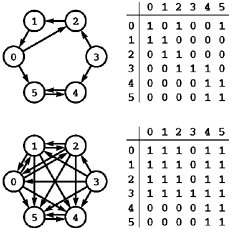
\includegraphics[scale=.7]{informatika/teoreticka_informatika/obrazky/tranzuzaver.png}
    \caption{Tranzitivn� uz�v�r grafu (zdroj: http://zorro.fme.vutbr.cz/graphs/foil36.html)}
  \end{center}
\end{figure}

\begin{e}{Pozn�mka}{0}{0}
  Plat�, �e matice dosa�itelnosti v grafu $G$ = matice sousednosti tranzitivn�ho
  uz�v�ru grafu $G$.
\end{e}

\begin{obecne}{Algoritmus}
Z ka�d�ho vrcholu vypustit DFS (Depth-first search~-- prohled�v�n� do hloubky), do spole�n� matice zaznamen�vat dosa�en� vrcholy (��dek odpov�d� vrcholu, sloupce vrchol�m, kter� jsou z n�ho dosa�iteln�) -- slo�itost $O(n(n+m))$.
\end{obecne}

\begin{obecne}{Warshall�v algoritmus}
Iterativn� konstrukce matice dosa�itelnosti, postupn� po��t� matice $W_k$, kde $w^{[k]}_{i, j} = 1$, pokud mezi vrcholy $i$ a $j$ existuje cesta, jej� v�echny vnit�n� vrcholy jsou mezi vrcholy $1\dots k$.

Z matice $W_k$ lze spo��tat matici $W^{[k+1]}: W^{[k+1]}_{i,j} = W^{[k]}_{i,j}  || (W^{[k]}_{i,k+1} \&\& W^{[k]}_{k+1,j})$ -- bu� vede mezi vrcholy $i, j$ cesta, kter� nepou�ije vrchol $k+1$, nebo takov�, kter� ho pou�ije -- v tom p��pad� ale mus� v�st cesty mezi vrcholy $i,k+1$ a $k+1,j$, kter� pou��vaj� pouze vrcholy $1\dots k$, jejich spojen�m je cesta mezi vrcholy $i,j$

Matice $W^1$ je matice incidence p�vodn�ho grafu.

Pseudok�d (vstup: I -- matice incidence, $[0,1]^{n\times n}$):
\begin{verbatim}
Procedure Warshall(I)
W:= I;
for k:=1 to n
begin
  for i:=1 to n
  begin
    for j:=1 to n
\end{verbatim}
      $w_{i,j} = w_{i,j} || (w_{i,k} \&\& w_{k,j})$
\begin{verbatim}
  end
end 
return W;
\end{verbatim}

Slo�itost algoritmu je jasn� $O(n^3)$ (pot�ebuje $2n^3$ bitov�ch operac�), co� m��e b�t lep�� pro grafy s hodn� hranami (po�et hran se bl�� $n^2$), ne� slo�itost $n*DFS$ ( $n*(n + m) \approx n * (n + n^2) = n^2 + n^3$ )

\end{obecne}

TODO: je�t� n�co?

\subsection{Algoritmy vyhled�v�n� v textu}
Toto s� len ve�mi stru�n� v��ahy z wikipedie. Aktu�lne s� tu len preto, aby si �lovek r�chlo vybavil, o �om tie algoritmy s� :-)

\subsubsection*{Rabin-Karp}
Umo��uje vyh�ad�vanie viacer�ch re�azcov v texte naraz - u�ito�n� napr. na h�adanie plagi�tov. Z�kladnou my�lienkou je vyh�ad�vanie v texte pomocou hashov (rolling hashes - idea je \texttt{s[i+1..i+m] = s[i..i+m-1] - s[i] + s[i+m]})...

Algoritmus pre vyh�ad�vanie jedn�ho re�azca:
\begin{verbatim}
 1 function RabinKarp(string s[1..n], string sub[1..m])
 2     hsub := hash(sub[1..m])
 3     hs := hash(s[1..m])
 4     for i from 1 to n-m+1
 5         if hs = hsub
 6             if s[i..i+m-1] = sub
 7                 return i
 8         hs := hash(s[i+1..i+m])
 9     return not found
\end{verbatim}

Najhor�ia zlo�itos� je $\Omega(mn)$. Pri vyh�ad�van� viacer�ch re�azcov len spo��tame hashe v�ek�ch h�adan�ch stringov a pri n�jden� niektor�ho z hashov pr�slu�n� re�azec porovn�me s textom... Ostatn� algoritmy spotrebuj� �as $O(n)$ na n�jdenie 1 re�azca a teda $O(nk)$ na vyh�adanie $k$ re�azcov. Naproti tomu tento algoritmus m� o�ak�van� zlo�itos� $O(n+k)$ - preto�e vyh�ad�vanie v hashovacej tabu�ke, �i je hash podre�azca textu rovn� hashu niektor�ho z h�adan�ho re�azcov, trv� $O(1)$.

\subsubsection*{Aho-Corasick}

Dok�e vyh�ad�va� viacero re�azcov naraz - pou��va na to trie-like �trukt�ru (kone�n� automat), ktor� obsahuje nasleduj�ce \uv{prvky}:
\begin{penumerate}
	\item kone�n� mno�ina $Q$ - stavy
	\item kone�n� abeceda $A$
	\item transition funkcia $g$: $Q \times A \rightarrow Q + \{fail\}$
	\item failure funkcia $h$: $Q \rightarrow Q + \{fail\}$. $h(q)=q'$ pr�ve vtedy ke� spomedzi v�etk�ch stavov Q d�va $q'$ najdlh�� suffix z $path(q)$.
	\item kone�n� mno�ina $F$ - koncov� stavy
\end{penumerate}

Pr�klad \uv{hotov�ho} automatu pre slov� P=\{ab, ba, babb, bb\}:

\par\begin{center}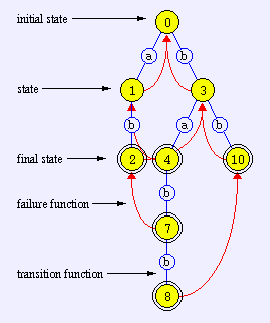
\includegraphics[width=8cm]{informatika/algoritmy_a_ds/obrazky/ahocorasick-automatron.png}\end{center}

Zlo�itos� vyh�ad�vania je line�rna vzh�adom k d�ke textu a po�tu n�jden�ch \uv{slov} (pozn.: ten m��e by� a� kvadradick� - slovn�k a, aa, aaa, aaaa; re�azec aaaa). Trie �trukt�ru je mo�n� vyrobi� raz a potom pou��va� po�as vyh�ad�vania - uchov�vame si najdl�� match a pou��vame suffix odkazy (aby sme udr�ali linearitu v�po�tu).

V�stavba stromu se provede prost�m za�azov�n�m slov do trie-stromu podle prefix�. Na t�to struktu�e je potom mo�n� v line�rn�m �ase (vzhledem k po�tu znak� hledan�ch slov) p�edpo��tat hodnoty failure funkce: automat v�dy pust�me na sufix aktu�ln� zkou�en�ho slova, bez prvn�ho znaku. D�ky tomu, �e pr�b�n� ukl�d�me hodnoty nalezen�ch slov, pro ka�d� p�smeno provede max. 2 kroky (postup vp�ed a ulo�en� hodnoty, kam bych spadnul).


\subsubsection*{Knuth-Morris-Pratt}

Obdoba Aho-Corasick, ale h�ad� len jedno slovo. Samozrejme nie je potrebn� dopredn� funkcia (v�dy iba nasleduj�ci znak), pou��va sa \uv{partial match} tabu�ka (failure funkcia).

\begin{verbatim}
algorithm kmp_search:
    input:
        S (the text to be searched)
        W (the word sought)

    m = 0 (the beginning of the current match in S)
    i = 0 (the position of the current character in W)
    an array of integers, T (the table, computed elsewhere)

    while m + i is less than the length of S, do:
        if W[i] = S[m + i],
            i = i + 1
            if i equals the length of W,
                return m
        otherwise,
            m = m + i - T[i],
            if i is greater than 0,
                i = T[i]

    (if we reach here, we have searched all of S unsuccessfully)
    return the length of S
\end{verbatim}

Zlo�itos� algoritmu je je $O(k)$ (k je d�ka S) - cyklus je vykonan� najviac $2k$ kr�t.

Algoritmus na v�robu tabu�ky:
\begin{verbatim}
algorithm kmp_table:
    input:
        W (the word to be analyzed)
        T (the table to be filled)

    i = 2 (the current position we are computing in T)
    j = 0 (the zero-based index in W of the next
           character of the current candidate substring)

    (the first few values are fixed but different
          from what the algorithm might suggest)
    let T[0] = -1
    T[1] = 0

    while i is less than the length of W, do:
        (first case: the substring continues)
        if W[i - 1] = W[j],
            T[i] = j + 1
            i = i + 1
            j = j + 1

        (second case: it doesn't, but we can fall back)
        otherwise, if j > 0,
            j = T[j]

        (third case: we have run out of candidates. Note j = 0)
        otherwise,
            T[i] = 0
            i = i + 1
\end{verbatim}


Zlo�itos� tohoto algoritmu je $O(n)$ (n je d�ka W) - cyklus skon�� najviac po $2n$ iter�ci�ch.

\subsection{Algebraick� algoritmy}

\subsubsection*{Diskr�tn� Fourierova Transformace (DFT)}

Diskr�tn� Fourierova transformace se pou��v�, chceme-li zachytit hodnotu (p�epokl�dejme, �e $2\pi$-periodick�) funkce na intervalu $[-\pi,\pi]$ v n�jak�ch $n$ bodech. To je dobr� nap�. pro vzorkov�n� elektrick�ho nebo zvukov�ho sign�lu a jin� operace. Pro n�jakou funkci n�m tak sta�� zn�t vektor dimenze $n$ (a $n$ je po�et vzork� na $2\pi$).

Je to zalo�eno na Fourierov�ch �ad�ch -- d� se uk�zat, �e funkce $1$, $\cos kx$ a $\sin kx$ pro $k\geq 1$ tvo�� ortogon�ln� b�zi prostoru spojit�ch funkc� na intervalu $[-\pi,\pi]$. Proto�e pot�ebujeme zn�t jenom kone�n� po�et vzork�, sta�� n�m jen kone�n� podprostor s kone�nou b�z�. M�me-li rozklad n�jak� $2\pi$-periodick� funkce do Fourierovy �ady $f(x)= c + \sum_{k=1}^\infty a_k \sin k x + \sum_{k=1}^\infty b_k \cos k x$, d� se jednodu�e uk�zat, �e pro hodnoty v bodech $-\pi,-\pi + \frac{\pi}{n}, -\pi + 2\frac{\pi}{n}, \dots, -\pi + (n-1)\frac{\pi}{n}$ sta�� sumy do $\frac{n}{2}-1$ pro sinusov� �ady a $\frac{n}{2}$ pro kosinov� -- vy��� koeficienty v takov�ch bodech jsou nulov�. Tak�e $n$ hodnot funkce $f$ na intervalu $[-\pi,\pi]$ lze reprezentovat vektorem $n$ ��sel v b�zi $1,\cos x,\dots,\cos \frac{n}{2}x,\sin x,\dots,\sin(\frac{n}{2}-1)x$. 

Jednodu�eji to lze uk�zat v komplexn�ch ��slech -- je zn�mo, �e 
$$e^{ix} = \cos x+ i\cdot\sin x$$
tak�e vektor hodnot funkce lze ekvivalentn� reprezentovat v b�zi $e^{i\cdot 2\pi\frac{k}{n}},\ k\in\{0,\dots,n\}$, nebo� v�echny vektory p�vodn� b�ze lze zapsat jako line�rn� kombinace vektor� nov� b�ze. Definujeme hodnotu
$$\omega := e^{i\cdot 2\pi\frac{1}{n}} \textrm{ (a to je vlastn� \uv{n�co jako} }\sqrt[n]{1}\textrm{)}$$
vid�me, �e $\omega^k$ je $n$-periodick� funkce, tak�e nez�le�� na hranic�ch sumace ($-\frac{n}{2}+1,\dots,\frac{n}{2}$ je ekvivalentn� $0,\dots,n-1$). 
Potom se posloupnost $n$ komplexn�ch ��sel $\alpha_0, \dots, \alpha_{n-1}$ (nap�. hodnot na�� funkce v bodech $-\pi + \frac{2\pi k}{n},\ k\in\{0,\dots,n-1\}$) transformuje na posloupnost $n$ komplexn�ch ��sel $A_0, \dots, A_{n-1}$ (do b�ze $\omega^i,\ i\in\{0,\dots,n-1\}$) pou�it�m vzore�ku:
$$A_j = \sum_{k=0}^{n-1} \alpha_k \omega^{kj}  \;\;\;\;\; j = 0, \dots, n-1$$
Tento p�evod ozna�ujeme jako \emph{diskr�tn� Fourierovu transformaci}.

\emph{Inverzn� diskr�tn� Fourierova transformace} je opa�n� probl�m -- z $n$ Fourierov�ch koeficient� $A_k$ chceme zp�tn� vypo��tat hodnoty funkce $\alpha_k$ v bodech $-\pi + \frac{2\pi k}{n},\ k\in\{0,\dots,n-1$. Plat�:

$$\alpha_j = \frac{1}{n}\sum_{k=0}^{n-1} A_k \omega^{-kj}  \;\;\;\;\; j = 0, \dots, n-1$$

\medskip
\begin{e}{D�kaz}{0}{0}
Definujeme matici $W: W_{p,q}=\omega^{pq}$, potom $A = W\alpha$ (vektorov�), tak�e $a = W^{-1}A$. Definujeme $W': W'_{p,q}=\omega^{-pq}$ a dok�eme, �e $W\cdot W'= n\cdot I_n$. M�me
$$(W\cdot W')_{p,q} = \sum_{s=0}^{n-1} W_{p,s}\cdot W'_{s,q} = \sum_{s=0}^{n-1} \omega^{(p-q)\cdot s}$$
a potom pro
\begin{pitemize}
    \item $p = q$ plat� $\sum_{s=0}^{n-1}\omega^{(p-q)\cdot s} = \sum_{s=0}^{n-1}\omega^0 = \sum_{s=0}^{n-1} 1 = n$
    \item $p\neq q$ definujeme
    $$Q:= \omega^{p-q}$$
    a dostaneme geometrickou posloupnost $Q^0 + Q^1 +\dots +Q^{n-1}$, pro jej� sou�et prvn�ch $n$ �len� plat� vzorec
    $$ \sum_{s=0}^{n-1} Q^s = Q^0 \frac{Q^{n-1+1} - 1}{Q-1} = 1\frac{1-1}{Q-1}= 0 $$
\end{pitemize}
\end{e}


\begin{e}{Algoritmus}{0}{Fast Fourier transform (FFT)}
Fast Fourier transform je algoritmus pro po��t�n� diskr�tn� Fourierovy transformace vektor� rozm�ru $n=2^k$ v �ase $\Theta(n\log n)$. M�m-li matici Fourierov�ch koeficient� $W, W_{p,q} = \alpha_q \omega^{pq}$, mohu ji rozd�lit na lich� a sud� sloupce, u sud�ch vyj�d�it $\omega^q$ a pro spodn� polovinu ��dek (se sumami jdouc�mi po dvou) mohu sn�it exponent u $\omega$ o $n/2$ (d�ky periodicit�) a vyjdou stejn� ��sla:
\begin{align*}
    A_j &= \sum_{k=0}^{n-1} \alpha_k \omega^{kj}\ &j\in\{0,\dots,n-1\}\\
    \\
    A_j &= \sum_{k=0}^{\frac{n}{2}-1} \alpha_{2k}\omega^{2kj} + \omega^j \sum_{k=0}^{\frac{n}{2}-1} \alpha_{2k+1}\omega^{2kj}\ &j\in\{0,\dots,\frac{n}{2}-1\}\\    
    A_{j+\frac{n}{2}} &= \sum_{k=0}^{\frac{n}{2}-1} \alpha_{2k}\omega^{2k(j+\frac{n}{2})} + \omega^{(j+\frac{n}{2})} \sum_{k=0}^{\frac{n}{2}-1} \alpha_{2k+1}\omega^{2k(j+\frac{n}{2})}\ &j\in\{0,\dots,\frac{n}{2}-1\}\\
\end{align*}

\textit{Pozn�mka: pro rychl� a jednoduch� pochopen� t�ch blekt� co jsem tu napsal doporu�uji Ku�er�v program Algovision}\\ \texttt{http://kam.mff.cuni.cz/\~{}ludek/AlgovisionPage.html} \\ \textit{DFT je tam n�zorn� a p�ehledn� uk�zan�.}
\end{e}

TODO: Souvisej�c� obecn� \uv{v�ci} o Fourierov� transofrmaci, pou�it� p�i spektr�ln� anal�ze (Nyquist-Shannon sampling theorem), datov� kompresi (Diskr�tn� kosinov� transformace), n�soben� polynom� (+n�soben� velk�ch integer�).

\subsubsection*{Euklid�v algoritmus}

Euklid�v algoritmus je postup (algoritmus), kter�m lze ur�it nejv�t��ho spole�n�ho d�litele dvou p�irozen�ch ��sel, tzn. nejvy��� ��slo takov�, �e beze zbytku d�l� ob� ��sla.

Algoritmus (pomoc� rekurze):
\begin{verbatim}
function gcd(a, b)
    if b = 0 return a
    else return gcd(b, a mod b)
\end{verbatim}

Algoritmus (pomoc� iterace):
\begin{verbatim}
function gcd(a, b)
    while b <> 0
        t := b
        b := a mod b
        a := t
    return a
\end{verbatim}

Algoritmus (jednoduch� ale neefektivn�):
\begin{verbatim}
function gcd(a, b)
    while b <> 0
        if a > b
            a := a - b
        else
            b := b - a
    return a
\end{verbatim}

Doba prov�d�n� programu je z�visl� na po�tu pr�chod� hlavn� smy�kou. Ten je maxim�ln� tehdy, jsou-li po��te�n� hodnoty u a v rovn� dv�ma po sob� jdouc�m �len�m Fibonacciho posloupnosti. Maxim�ln� po�et proveden�ch opakov�n� je tedy $\log_\phi (3-\phi)v \approx 4{,}785 \log v + 0{,}6273 = O(\log v)$. Pr�m�rn� po�et krok� pak je o n�co ni���, p�ibli�n� $\frac{12 \ln 2}{\pi^2}\log v \approx 1{,}9405 \log v = O(\log v)$.
\\\\
\begin{e}{Report}{0}{Skopal} DFT
\end{e}

\subsection{Z�klady kryptografie, RSA\sout{, DES}}

(nejsou zde uvedeny p��klady symetrick�ch �ifer, pro z�jemce vesel� komiks o AES -- \url{http://www.moserware.com/2009/09/stick-figure-guide-to-advanced.html} :))

\subsubsection*{Z�klady kryptografie\footnote{sestaveno podle vrazedneho zkouseni Jaghobem}} 
\begin{e}{Definice}{1}{Kryptografick� syst�m}
Prostor otev�en�ch zpr�v $M$, �ifrovan�ch zpr�v $C$, �ifrovac�ch a de�ifrovac�ch kl��� $K$ a $K'$. Efektivn� generov�n� kl���
                        $G:N\to K\times K'$, �ifrov�n� $E:M\times K\to C$, de�ifrov�n� $D:C\times K'\to M$.
\begin{pitemize}
  \item \textbf{Symetrick�} (sd�len� kl�� $k_e = k_d$) rychl�, kr�tk� kl��e, potreba menit klice a bezpecne si je vymenit
  \item\textbf{Asymetrick�} (ve�ejn� kl�� $k_e \neq k_d$) delsi klice a pomalejsi nez symetrick�, neni pot�eba tajn� v�m�na, neni pot�eba tak �asto m�nit kl��e 
\end{pitemize}                  
\end{e}

\begin{e}{Definice}{0}{Nahodn� gener�tory}
Pou��vaj� se pro generov�n� kl��� pro �ifry (nap� RSA) a v proudov�ch �ifr�ch.
\begin{pitemize}
  \item\textbf{HW} za��zen� �asto zalo�en� na jevech generuj�c�ch statisticky n�hodn� "�umov�" sign�ly, nap��klad z tepeln�ho �umu polovodi�e.
  \item\textbf{SW} jsou zalo�eny na pozorov�n� jev� v po��ta�i z hlediska programu n�hodn�ch, �asto z u�ivatelsk�ho vstupu (nap�. PuTTYgen pou��v� pro generov�n� RSA kl��e p�ej�zd�n� my��). 
  \item\textbf{Pseudon�hodn�} jsou deterministick� programy generuj�c� posloupnost ��sel pokud mo�no nerozli�itelnou od n�hodn�.
        \begin{pitemize}
                \item p�. kongruen�n� gener�tor: $X_{n+1} = ( a X_n + c ) \mod m$ 
                \item pou��vaj� se v proudov�ch �ifr�ch
        \end{pitemize}  
\end{pitemize} 
\end{e}

\begin{e}{Definice}{0}{Hashovaci funkce}
Funkci $h:U\rightarrow\{0,1,\dots,m-1\}$ naz�v�me \textbf{ha�ovac� funkc�}.\footnote{viz ot�zku Ha�ov�n�}
\\\\
\textbf{Po�adavky:}
\begin{pitemize}
  \item Rovnom�rn� a n�hodn� rozlo�en� hodnot
  \item Odolnost na kolize (v�po�etn� slo�it� naj�t pro $x\neq x$ $h(x)=h(y)$) 
  \item Jednosm�rn� funkce (v�po�etn� slo�it� naj�t $y$ k $x$ pro $h(x)=y$)     
  \item Efektivn� algoritmus
\end{pitemize} 
\textbf{Vyu�it�:}
CRC (kontroln� sou�et), ukl�d�n� hesel (MD5,SHA) ...      

\end{e}

\begin{e}{Definice}{0}{Model utocnika podle Doleva a Yao}
\begin{pitemize}
  \item M��e z�skat libovolnou zpr�vu putuj�c� po s�ti
  \item Je pr�voplatn�m u�ivatelem s�t� a tud� m��e zah�jit komunikaci s jin�m u�ivatelem
  \item M��e se st�t p��jemcem zpr�v kohokoliv
  \item M��e zas�lat zpr�vy komukoliv zosobn�n�m se za jin�ho u�ivatele
  \item Neumi rozume resit NP-uplne problemy (ani slozitejsi)\footnote{tzn. i slab��: Nem��e odhadnout n�hodn� ��slo z dostate�n� velk�ho prostoru}   
  \item Bez spr�vn�ho kl��e nem��e nal�zt zpr�vu k �ifrovan� zpr�v� a nem��e vytvo�it platnou �ifrovanou zpr�vu z dan� zpr�vy, v�e vzhledem k n�jak�mu �ifrovac�mu algoritmu 
\end{pitemize}  
\end{e}

\begin{e}{Definice}{0}{Cile utoku}
        \begin{description}
                \item\textbf{d�v�rnost dat} u�ivatel m��e ur�it kdo m� data vid�t, a syst�m skute�n� dovol� pracovat s daty pouze povolen�m u�ivatel�m
                \item\textbf{celistvost dat} mo�nost podstr�en� fale�n�ch dat
                \item\textbf{dostupnost syst�mu} \emph{DoS (Denial of Service)}
        \end{description}
\end{e}

\begin{e}{P��klad}{0}{0}
Ukazku pouziti nejakeho sifrovaciho protokolu (zvolil jsem kombinace symetricka sifra sifrovani, asymetricka predani klicu k symetricke).
\\\\TODO
\end{e}
\begin{e}{Definice}{0}{protokol Diffie-Hellman}
\begin{pitemize} 
\item Diffie-Hellman v�mena kl�cu je kryptografick� protokol, kter� umo�nuje nav�zat bezpecn� spojen�. Pro bezpecn� spojen� je potreba si vymenit kl�c k symetrick� �ifre pres je�te nezabezpecen� kan�l. Pr�ve tento protokol to umo�nuje ani� by byl kl�c jednodu�e posl�n v otevren� forme.
\item Alice si vymysl� velk� prvoc�slo $p$, gener�tor $g$ kone�n� grupy $G=(Z^*_p,\cdot)$
a $a\in[1,p-1)$ vypocte A po�le Bobovi [g,p,A], Bob vypocte B a po�le ho Alici oba si vypoc�taj� K $\Rightarrow$ muzou zacit symetricky sifrovanou komunikaci
\end{pitemize}

\begin{figure}
  \begin{center}
    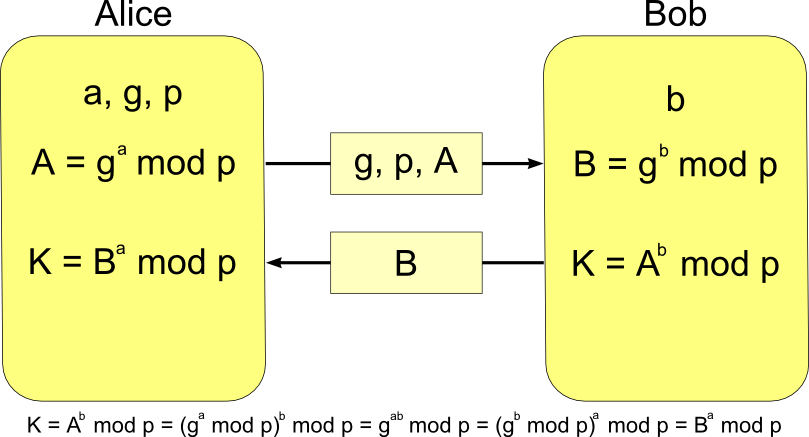
\includegraphics[width=10cm]{informatika/siete_a_bezpecnost/obrazky/dh-system.png}
    \caption{D-H protokol}
  \end{center}
\end{figure}

\begin{pitemize}
\item Puvodne nezabezpecoval autentifikaci ucastniku = nachylny k utoku man-in-the-middle. Man-in-the-middle muze vytvorit komunikaci s dvema ruznymi Diffie-Hellman klici, jeden s Alici a druhej s Bobem, a pak se tvarit jako Alice k Bobovi a obracene, treba pomoci dekodovani a rekodovani zprav mezi nimi. Nejaka metoda autentifikace mezi temito osobami je nutna.
\item Probl�mu nalezen� c�sla  a  ze znalosti ga  mod  p  se r�k� probl�m diskr�tn�ho logaritmu.  Tento probl�m je st�le pova�ov�n za velmi obt�n�. \end{pitemize} 

\end{e}

\subsubsection*{RSA (Rivest-Shamir-Adleman)}
Asymetrick� �ifra (r�zn� kl��e pro �ifrov�n� a de�ifrov�n�), pou�iteln� jako �ifra s�ve�ejn�m kl��em. Kryptosch�ma je zalo�eno na Eulerove formuli.
\\\\
Alice a Bob se verejne dohodnou na hranici $N$ a chtej� si vymenovat tajn� zpr�vy $0 \leq m<N$.
\textbf{Inicializace:}
\begin{penumerate}
        \item vybrat dv� dostate�n� velk� prvo��sla $p$, $q$ tak aby $n= p\cdot q < N$
        \item Alice spo��t� $\varphi(n) = (p-1)\cdot (q-1)$\\ 
        (Eulerova funkce $\varphi(n)$ je po�et ��sel men��ch ne� $n$, kter� jsou s $n$ nesoud�ln�)
        \item vybrat $e$ takov�, �e $1 < e < \varphi(n)$ a $e$ je nesoud�ln� s $\varphi(n)$\\ -- dvojice ($n,e$) bude \emph{ve�ejn� kl�� (public key)}
        \item vybrat $d$ tak, aby 
                $$d\cdot e \equiv 1 \mod \varphi(n)$$ 
                takov� $d$ lze naj�t roz���en�m euklidov�m algoritmem\\
                -- dvojice ($n,d$) bude \emph{de�ifrovac� kl�� (private key)}
\end{penumerate}

\textbf{�ifrov�n�:}
\begin{penumerate}
        \item Alice pos�l� public key Bobovi (��sla $n$ a $e$), nech�v� si private key
        \item Bob chce Alici poslat zpr�vu $m$ tak spo��t� :
                $$c = m^e \mod n$$
        \item Bob ode�le $c$ Alici
\end{penumerate}

\textbf{De�ifrov�n�:}
\begin{penumerate}
\item Alice p�ijala $c$
\item Spo��t�:
        $$m = c^d \mod n$$
\end{penumerate}

�ifra (to, �e to v�bec funguje, tedy, �e $m = (m^e)^d$) se op�r� o n�kolik netrivi�ln�ch v�t algebry...
\begin{pitemize}
\item Pro re�ln� pou�it� c�sla pribli�ne 100 a� 200 bitu. Kl�c e vol�me jako prvoc�slo vet�� ne� $(p - 1)$ a $(q � 1)$. Hranice bezpecnosti pro modul n je $N$ = 1024 bitu, rozumn� 1500 bitu, l�pe 2048
\item Nen� zn�ma metoda vedouc� k rozbit� tohoto algoritmu
\item Slabost� je hypotetick� mo�nost vytvorit elektronick� podpis zpr�vy bez znalosti de�ifrovac�ho kl�ce na z�klade zachycen� vhodn�ch predchoz�ch za�ifrovan�ch zpr�v.
\item nap��klad SSH protokol pou��v� RSA kl��e
\end{pitemize}

\begin{e}{Report}{0}{Skopal} RSA, DES (tady cht�l Skopal konkr�tn� vzore�ky, jak funguje symetrick� �ifra nebo �ifrov�n� s v��ejn�m kl��em ho nez�j�malo)
\end{e}

\begin{e}{Report}{0}{Yaghob}
Vedom si nebezpecnosti situace nabidl jsem p. Yaghobovi "sestaveni nakupniho kosiku". Povedel jsem, ze by se k tematu dala povedet hromada veci, tak jestli bychom se mohli domluvit na podmnozine ktera jej zajima, at zbytecne neplnim papir. Souhlasil nacez jsem mu nabidl hromadu vice ci mene souvisejicich veci, pridal par hodne vlastnich.
\\\\Nechtel: S-Box, RSA,DES ani zadnou konkretni sifru, konkretni metody utoku, obranu proti utokum, pravidla pro volbu dobreho hesla, steganografii, proudove sifry,historii...
\\\\Chtel:

    Formalne popsat kryptograficky system - bacha! tady bylo videt, ze jde o klicovy pojem, kdyz ho clovek neformuluje - tak (nejspis) konci.

    Nahodne generatory + vlastnosti, ktere od nich chceme + zhruba algoritmicky princip (an = (an-1*b+c) mod d)) + kde se pouziji (generovani klicu)
    
    Hashovaci funkce + vlastnosti, ktere od nich chceme, kde se pouziji (crc, neukladat hesla v plaintextu, ...)
    
    Model utocnika podle Doleva a Yao (pozor! v materialech napsano: neumi uhodnout nah.cislo z dost velke mnoziny, spravne je obecnejsi: Neumi rozume resit NP-uplne problemy (ani slozitejsi (: )).
    
    Cile utoku
    
    Ukazku pouziti nejakeho sifrovaciho protokolu (zvolil jsem kombinace symetricka sifra sifrovani, asymetricka predani klicu k symetricke).
    
    Vymenu klicu a-la Diffie Hellman
    
    Pokud jsem neco nevedel, dostal jsem cas na premysleni, pripadne jemne natuknuti. Veci chtel hodne formalne.
    
    Nemit Ochranu informace I a II + vlastni zajem o oblast, tak certain doom!
\end{e}

\subsection{Pravd�podobostn� algoritmy -- testov�n� prvo��selnosti\footnote{tato ot�zka nebyla asi nikdy zkou�ena, a tak je to jenom takovy n�st�el Zdroj: v�born� �epkovy slajdy na ADS2 - zda se ze je ocenuju az ted :)}}

Pravd�podobnostn� (n�hodnostn�) algoritmy jsou nedeterministick� algoritmy, kter� se sna�� naj�t �e�en� rychleji nebo �e�en� t�ko �e�iteln�ch probl�m�, �asto NP-�pln�ch probl�m�. Pravd�podobnostn� algoritmus se m��e n�hodn� rozhodovat mezi r�zn�mi mo�nostmi jak pokra�ovat. Pro stejn� vstup m��e d�vat takov� algoritmus r�zn� v�sledky, kter� mohou b�t dokonce nespr�vn�. Mnohdy se tedy na dan�m vstupu spust� pravd�podobnostn� algoritmus v�cekr�t, aby se s v�t�� pravd�podobnost� dosp�lo ke spr�vn�mu v�sledku.
\\\\
Pravd�podobnostn�ch algoritm� je mnoho typ�, zde zm�n�me jen dva a to algoritmy typu Las Vegas a typu Monte Carlo. 

\subsubsection*{Algoritmy typu Las Vegas} 
V�sledek je v�dy spr�vn�, n�hodnost ovliv�uje pouze dobu b�hu algoritmu, tj. po jak� cest� se algoritmus ke spr�vn�mu v�sledku dobere.
\\\\ 
\begin{prikladN}{randomizovan� QuickSort} Od deterministick� verze se li�� n�hodn�mi v�b�ry pivota p�i ka�d�m d�len� posloupnosti, co� poskytuje n�sleduj�c� v�hody
\begin{pitemize}
\item d�v� dobr� pr�m�rn� �as (tj. $O(n \log n)$) i v p��pad�, �e data na vstupu nejsou n�hodn� permutace � ��dn� vstup nen� apriori �patn� (pro ka�d� deterministick� v�b�r pivota existuj� apriori �patn� vstupy)
\item m��e b�t spu�t�n paraleln� v n�kolika kopi�ch, v�sledek je z�sk�n z kopie, kde v�po�et skon�� nejd��ve (pro deterministickou verzi nem� takov� postup ��dn� smysl)
\end{pitemize}
\end{prikladN}
\subsubsection*{Algoritmy typu Monte Carlo} 
N�hodnost ovliv�uje jak dobu b�hu, tak spr�vnost v�sledku: algoritmus m��e ud�lat chybu, ale pouze jednostrann� (u odpov�d� ANO/NE) a s omezenou pravd�podobnost�. 
\\\\
\begin{prikladN}{Rabin-Miller�v algoritmus na testov�n� prvo��selnosti} 
Pro zadan� p�irozen� ��slo n (rychle) rozhodnout zda je n prvo��slo 
\\\\
\begin{e} \equiv 1(\mod p)${V�ta}{0}{Mal� Fermatova} Nech� p je prvo��slo. Potom $\forall k \in\{1,2, � ,p-1\}$ plat� $k^{p-1}
\end{e} 
\\\noindent
Pokud $n$ nen� prvo��slo, tak zkus�me (n�hodn�) naj�t �sv�dka� $k$, poru�uj�c�ho $k^{n-1} \equiv 1(\mod n)$, kter� �dosv�d�uje�, �e $n$ je opravdu ��slo slo�en� (nen� to prvo��slo). Probl�m - pro n�kter� slo�en� ��sla je sv�dk� p��li� m�lo, tak�e je p��li� mal� pravd�podobnost, �e n�jak�ho sv�dka (n�hodn�) vybereme. 
\\\\
\begin{e} Nech� T je mno�ina dvojic p�irozen�ch ��sel, kde $(k,n) \in T$ pokud $0 < k < n$ a je spln�na alespo� jedna z n�sleduj�c�ch dvou podm�nek:\\{Definice}{0}{0}
1. neplat� $k^{n-1} \equiv 1(\mod n)$,\\
2. existuje $i$ takov�, �e $m = (n-1) / 2^i$ je p�irozen� ��slo a plat� $1 < NSD(k^{m-1}-1, n) < n$ 
\end{e}
\begin{e} ��slo $n$ je slo�en� tehdy a jen tehdy, kdy� existuje $k$ takov�, �e $(k,n)\in T$.{V�ta}{0}{1}
\end{e}
\begin{e} Nech� $n$ je slo�en� ��slo. Pak existuje alespo� $(n-1)/2$ takov�ch ��sel $k$, pro kter� plat� $(k,n)\in T$.{V�ta}{0}{2}
\end{e}
\begin{obecne}{Algoritmus:}
\begin{verbatim}
        Rabin-Miller(n); 
                for i:=1 to po�et do 
                        ki := n�hodn� p�irozen� ��slo z intervalu [1,n-1];
                        if (ki,n) in T then Return(n je slo�en�);                
                Return(n je prvo��slo)
\end{verbatim}
\end{obecne}
\noindent
Pokud $Rabin-Miller(n)$ rozhodne, �e $n$ je slo�en�, tak je to zaru�en� spr�vn� v�sledek (byl nalezen �sv�dek�), pokud $Rabin-Miller(n)$ rozhodne, �e $n$ je prvo��slo, tak se m��e jednat o chybu, ale pouze v p��pad�, �e v�echna vybran� $k_i$ byli �ne-sv�dci� pro slo�en� ��slo $n$, co� ale m��e (d�ky V�t� 2) nastat nejv��e s pravd�podobnost� $$P(chyba) \leq (1/2)^{pocet}$$ pokud jsou v�b�ry jednotliv�ch $k_i$ vz�jemn� nez�visl� 
\\\\
\begin{obecne}{Vlastnosti algoritmu:}
� zvy�ov�n�m po�tu iterac� (po�tu testovan�ch $k_i$) lze dostat libovoln� malou (p�edem zvolenou) pravd�podobnost chyby
\\
� jednotliv� iterace (testy pro r�zn� $k_i$) lze prov�d�t paraleln� 
\end{obecne}
\begin{obecne}{�asov� slo�itost:} ka�d� iterace trv� jen polynomi�ln� vzhledem k d�lce z�pisu ��sla $n$ (tj. k d�lce vstupu), k tomu je ov�em pot�eba uk�zat, �e test zda $(k_i,n) \in T$ je mo�no prov�st v �ase polynomi�ln�m v $\log n$, co� nen� trivi�ln� (je nutn� m�t dal�� znalosti z teorie ��sel)
\end{obecne}
\end{prikladN}


\subsection{Aproxima�n� algoritmy}
(tato ot�zka asi nebyla nikdy zkou�ena tak�e je to jenom takov� n�st�el, asi m� cenu seto  u�it a� kdy� pochop�te NP-�pln� probl�my (hlavn� kliku a rozvrh) Zdroj: �epkovy slajdy na ADS2)

Aprox. algoritmy jsou vhodn� tam, kde je nalezen� optim�ln�ho �e�en� �beznad�jn� (�asov� p��li� n�ro�n�), typicky u NP-t�k�ch optimaliza�n�ch �loh (optimaliza�n�ch verz� NP-�pln�ch rozhodovac�ch probl�m�). Maj� n�sleduj�c� t�i vlastnosti:
\\1. konstruuj� suboptim�ln� �e�en�
\\2. poskytuj� odhad kvality zkonstruovan�ho �e�en� vzhledem k optimu
\\3. b�� v polynomi�ln�m �ase (jinak nejsou zaj�mav�) 
\\\\
\begin{e}{P��klad}{0}{maximaliza�n� �lohy (optimaliza�n� verze KLIKY)} Pro dan� neorientovan� graf najdi nejv�t�� (po�tem vrchol�) kliku (�pln� podgraf). Po aproxima�n�m algoritmu chceme garanci typu $f(APROX) \geq \frac3 4 f(OPT)$, kde $f(X)$ je v tomto p��pad� po�et vrchol� (tj. velikost kliky) v �e�en� X, OPT je optim�ln� �e�en� a APROX je �e�en� vydan� aproxima�n�m algoritmem.
\end{e}
\begin{e} {P��klad}{0}{P��klad minimaliza�n� �lohy (optimaliza�n� verze ROZ)} Rozvrh na paralel. stroj�ch. Pro dan� �koly a dan� po�et stroj� najdi nejkrat�� rozvrh. Po aproxima�n�m algoritmu chceme garanci typu $f(APROX) \leq 2 f(OPT)$.
\end{e}
\begin{e}{Definice}{0}{0} \textit{Chyba aproxima�n�ho algoritmu} je definov�na jako pom�r (pod�l) $f(APROX) / f(OPT)$ pro minimaliza�n� �lohy a $f(OPT) / f(APROX)$ pro maximaliza�n� �lohy. Relativn� chyba je pak definov�na jako $|f(APROX) f(OPT)| / f(OPT)$.
\end{e}
\begin{e}{Algoritmus}{0}{Naivn� aproxima�n� algoritmus $FRONTA$} pro optimaliza�n� verzi $ROZ$: bere �koly postupn� podle jejich ��sel a ka�d� �kol v�dy um�st� na stroj, kter� je voln� nejd��ve. 
\end{e}
\begin{obecne}{Zna�en�:} $OPT$ = optim�ln� rozvrh, $Q$ = rozvrh zkonstruovan� algoritmem FRONTA, d�lka(OPT) = $o$, d�lka(Q) = $q$ 
\end{obecne}
\begin{e}{V�ta}{0}{0} Pokud m je po�et stroj�, tak $q \leq ((2m- 1) / m)o$ a tento odhad ji� nelze zlep�it.
\proof
d�kazy v�ech v�t z t�to kapitoly najdete t�eba u hippiese: \\\url{http://hippies.matfyz.info/poznamky/predmet_ads2/gallery.php?ID=28}
\end{e}

\begin{e}{D�sledek}{0}{0} Aproxima�n� algoritmus FRONTA m� pom�rovou chybu 2. 
\proof
1.T�snost odhadu: Pro ka�d� $m$ zkonstruujeme zad�n�, pro kter� plat� v dokazovan� nerovnosti rovnost, a to n�sleduj�c�m zp�sobem \\
$x_1 = x_2 = � = x_{m-1} = m-1$ ($m-1$ �kol� d�lky $m-1$) \\
$x_m = x_{m+1} = � = x_{2m-2} = 1$ ($m-1$ �kol� d�lky $1$) \\
$x_{2m-1} = m$ (1 �kol d�lky $m$)
\\2.Platnost nerovnosti: Nech� $j$ je �kol kon��c� jako posledn� v rozvrhu $Q$ (kon��c� v �ase $q$) a nech� $t$ je okam�ik zah�jen� �kolu $j$. Potom ��dn� procesor nem� prostoj p�ed �asem $t$ a plat� $mq \leq (2m-1)o$ .
\end{e}
\begin{e}{Algoritmus}{0}{Lep�� aproxima�n� algoritmus USPO��DAN� FRONTA} pro optimaliza�n� verzi ROZ: pracuje stejn� jako FRONTA, ale na za��tku �koly set��d� do nerostouc� posloupnosti podle jejich d�lek. 
\end{e}
\begin{obecne}{Zna�en�:} 
OPT = optim�ln� rozvrh, 
\\U = rozvrh zkonstruovan� algoritmem USPO��DAN� FRONTA, 
\\d�lka(OPT) = o, d�lka(U) = u 
\end{obecne}
\begin{e}{V�ta}{0}{0} Pokud $m$ je po�et stroj�, tak $u \leq ((4m - 1) / 3m)o$ a tento odhad ji� nelze zlep�it. 
\end{e}
\begin{e}{D�sledek}{0}{0} Aproxima�n� algoritmus USPO��DAN� FRONTA m� pom�rovou chybu $4/3$. 
\proof T�snost odhadu: Pro ka�d� lich� $m$ zkonstruujeme zad�n�, pro kter� plat� v dokazovan� nerovnosti rovnost, a to n�sleduj�c�m zp�sobem 
\\$x_1 = x_2 = 2m-1$ (2 �koly d�lky $2m-1$) 
\\$x_3 = x_4 = 2m-2$ (2 �koly d�lky $2m-2$) 
\\$x_{2m-3} = x_{2m-2} = m+1$ (2 �koly d�lky $m+1$) 
\\$x_{2m-1} = x_{2m} = x_{2m+1} = m$ (3 �koly d�lky $m$) 
\end{e}
\begin{e}{Lemma}{0}{0} Pokud pro v�echny �koly plat� $x_i \leq 1/3o$ pak $u = o$. \end{e}
\noindent\emph{Dokon�en� d�kazu:} Nech� $j$ je �kol kon��c� jako posledn� v rozvrhu $U$ (kon��c� v �ase $u$). Pokud $x_j > 1/3o$ tak pou�ijeme Lemma, v opa�n�m p��pad� je d�kaz velmi podobn� jako pro algoritmus FRONTA.
\end{obecne}


\end{document}
